\documentclass[aoas,preprint]{imsart}
%\pdfoutput=1    % Make arXiv happy

\RequirePackage[OT1]{fontenc}
\RequirePackage{amsthm,amsmath,amssymb}
\RequirePackage[colorlinks,citecolor=blue,urlcolor=blue]{hyperref}
\RequirePackage{hypernat}
\RequirePackage{graphicx}
\RequirePackage{enumerate}
\RequirePackage{booktabs}
\RequirePackage{subfigure}
\belowbottomsep=0.5em

\setattribute{journal}{name}{}  % Suppress text "Submitted to..."

\startlocaldefs
\usepackage{iproc-macros}
\endlocaldefs


\begin{document}

\begin{frontmatter}

\title{%
    Consistent partial-likelihood
    %Maximum-likelihood
    inference for directed interaction data with covariates
    %A model for repeated interactions with applications to e-mail traffic
    %analysis%
    \protect\thanksref{T1}
}

\runtitle{Inference for directed interaction data}
\thankstext{T1}{Work supported in part by the Army Research Office under PECASE Award W911NF-09-1-0555 and by the Office of Naval Research under MURI Award 58153-MA-MUR.}

\begin{aug}
    \author{%
        \fnms{Patrick O.} \snm{Perry}\corref{}%
        \ead[label=e1]{patperry@seas.harvard.edu}%
    }%
    \and%
    \author{%
        \fnms{Patrick J.} \snm{Wolfe}%
        \ead[label=e2]{wolfe@stat.harvard.edu}%
    }%

    \runauthor{P.\ O.\ Perry and P.\ J.\ Wolfe}

    \affiliation{Harvard University}

    \address{
        Statistics and Information Sciences Laboratory \\
        Harvard University \\
        33 Oxford Street \\
        Cambridge, MA 02138 \\
        \printead{e1}\\
        \phantom{E-mail:\ }\printead*{e2}
    }
\end{aug}

\begin{abstract}
Data derived from repeated directed interactions amongst entities are fast becoming
common in statistical analysis, communications networks being one canonical example.  Here we consider partial-likelihood inference for the general case of directed interaction data in the presence of covariates.  We model these interactions in continuous time as a point process, by way of a Cox multiplicative intensity model to adjust for reciprocation effects and obtain accurate
estimates of group-level *** social behavior.  We prove that the estimation
procedure is asymptotically consistent as the time increases.  We also prove
that improper handling of interactions between more than two individuals
leads to bias in the estimates, and we show how to correct the bias.  Our
motivating example is estimating gender-level e-mail preferences in a
corporate e-mail network.

We give conditions under which the bias can be corrected.

*** And also describe an efficient implementation of the resulting inference and bootstrap procedures.
\end{abstract}

\begin{keyword}[class=AMS]
    \kwd[Primary ]{62M30}     % Statistics:Inference from stochastic processes:Spatial processes
    \kwd[; secondary ]{62N01} % Statistics:Survival analysis and censored data:Censored data models
\end{keyword}

\begin{keyword}
    \kwd{random graphs}
    \kwd{networks}
    \kwd{point processes}
    \kwd{inference}
\end{keyword}

\end{frontmatter}


\section{Introduction}

Networks of relational data are fast becoming more prevalent, and therefore an increasingly pressing subject of scientific and statistical enquiry.  While such networks are typically framed as ``ties'' between entities, it is often the case in practice that network observables comprise counts of interactions between individuals or groups tabulated over time.  Modern-day communications networks give rise to important examples of \emph{directed} interactions: phone calls, text messages, or e-mails exchanged amongst a given set of individuals over a specific time period \cite{eagle2006reality,tyler2005email}.  Other examples of interactions include animal association patterns (for instance, zebras congregate at locations in their habitat \cite{sundaresan2007network}); gang homicides (e.g., gangs in Chicago murder members of rival factions \cite{papachristos2009murder}; legislation cosponsorship (legislators author bills, which others then sponsor \cite{fowler2006connecting}); and migration patterns (for example, families migrate between communities in Mexico \cite{mckenzie2007network}).

In this article, we consider partial-likelihood inference for the general case of directed interaction data in the presence of covariates.  We first develop the theory for the case in which interactions are strictly pairwise, and then generalize our results to the multiple-interaction case; we also provide efficient algorithms for partial likelihood maximization in these settings.  Our main assumptions are that the interactions are instantaneous; that the corresponding stochastic intensities used to model them are formally predictable and continuous; and that any covariates are locally bounded and predictable.

The interaction datasets we consider comprise a set of triples $(t,i,j)$ indicating that at time $t$, the directed interaction $i\rightarrow j$ took place; for instance, individual $i$ e-mailed individual $j$.  Given a set of such triples and covariate information about the corresponding initiators and receivers, a primary modeling goal is to determine which characteristics and behaviors are predictive of interaction.  In this vein, at least two questions are relevant:

\begin{enumerate}
    \item Is a shared attribute between entities predictive of increased
    interaction?

    \item If entity $i$ initiates an interaction with entity $j$, is this
    associated with $j$ being more likely to interact with $i$ in the future?
    If so, how does this effect decay with time?
\end{enumerate}

%We begin with a motivating example:

In the remainder of this article, we provide a modeling framework and efficient maximum-likelihood inference procedures to facilitate an analysis of such questions.  Section~\ref{S:model-elicitation} elicits a model appropriate for directed interactions.
Section~\ref{S:point-process-model} presents the basic multiplicative
intensity model,
Section~\ref{S:multiple-receivers} discusses extensions for multiple
receivers, and Sections~\ref{S:enron-modeling}~and~\ref{S:gender-bias}
present the results of fitting the model to the e-mail network.  We
prove asymptotic consistency for the single-receiver setting in
Section~\ref{S:MPLE-consistency}, and investigate bias in the multiple
receiver setting in Section~\ref{S:bias-correction}.
Section~\ref{S:discussion} concludes with discussion; further details and
proof of the theorems are provided in the appendices.

\section{Model Elicitation}\label{S:model-elicitation}

In studying human behavior, Sociologists repeatedly find evidence of homophily,
the tendency of individuals to associate with similar others
\cite{mcpherson2001birds}. A typical inquiry is to see if people with identical
genders interact more often then people with differing genders.  For instance, in a standard dataset comprising 4 years of e-mail exchanges amongst members of the Enron corporation (see Appendix~\ref{S:enron-corpus}), one might wish to test for gender bias in both group-level behaviors. The relevant data are summarized in Table~\ref{T:gender-send-counts},
\begin{table}[t]
    
\begin{tabular}{lrr}
    \toprule
    & \multicolumn{2}{c}{\textbf{To}} \\
    \cmidrule(l){2-3}
    \textbf{From} & Female & Male  \\
    \midrule
    Female&7529&8061 \\
    Male&5310&17488 \\
    \bottomrule
\end{tabular}

    \caption{
        Directed interactions (21,635 e-mails) among 43 female and 114 male Enron employees; multiple-recipient messages are tabulated as separate pairwise interactions (38,388 total).
    }
    \label{T:gender-send-counts}
\end{table}
if we treat the messages as independent and identically distributed observations,
then any reasonable test will find gender bias in both group-level behaviors.
Given that a female is sending a message, the probability that the recipient
is male will be estimated to be about 0.48, with a standard error around
0.004; given that a male is sending a message, the estimate will be about
0.23 with a standard error around 0.002.  Since these proportions fail to agree with the proportions of 28\% female and 72\% male employees, we would apparently conclude that bias is present in each group, associated with higher
within-group sending rates.

There are three main problems with this simple analysis:
\begin{enumerate}
    \item \textbf{Self-interactions may be excluded.} In the language of contingency table analysis, there may be ``structural zeros'' along the main *** diagonal of the table; this is well known to preclude closed-form maximum likelihood estimates even under simple models.\footnote{In network terminology, ``self-loops'' may be excluded; this often results in an approximate maximum-likelihood analysis.}

    \item \textbf{Interactions cannot necessarily be assumed independent.} For instance, as we show in Section~\ref{**}, we may wish to test for group-level reciprocation effects: whether or not recent interactions are predictive of future interactions.

    \item \textbf{Interactions may not be strictly pairwise.} As we show in Section~\ref{**}, treating extra-dyadic interactions as separate pairwise ones in general leads to bias in parameter estimates.
\end{enumerate}
The first issue is easy to fix, but the other two require significant
attention.

***

Traditionally, count data such as these are treated via contingency table analysis; in the presence of covariates, log-linear models are often used.

Consider the example of data derived from a communications network:

As far as we are aware, this is the first time that such machinery has been brought to bear on network-style relational data.

***

In the motivating example of e-mail exchanges given above, 1) corresponds to the fact that users do not typically interact with themselves via e-mail; 2) to the fact that if $i$ sends $j$ a message today, $j$ is more likely to send to $i$ tomorrow---any inherent gender bias will be exaggerated by reciprocation effects; and 3) is evidenced by the fact that more than 30\% of the messages in the Enron dataset have more than one recipient.


\begin{figure}
    %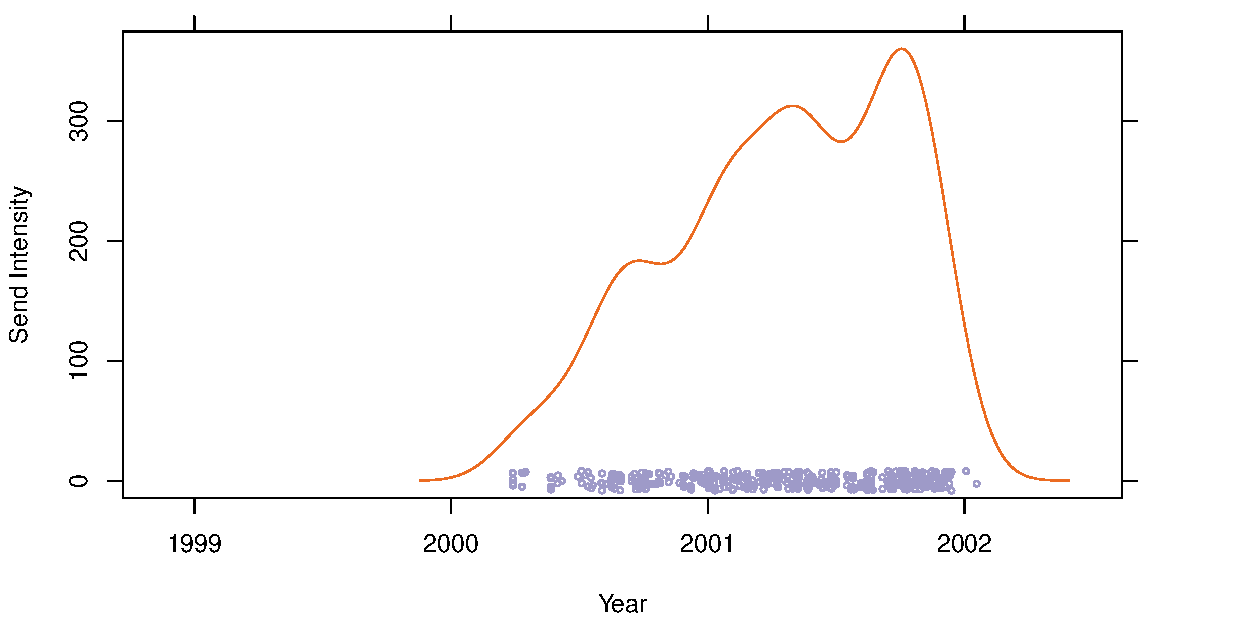
\includegraphics[scale=0.6]{figures/kernel-intensity}
    \caption{
        \textsc{Messages sent by the first employee in the Enron dataset.}
        Each of the 413 messages sent by the employee is represented by a point
        whose $x$ value is the time of the message and whose $y$ value is a
        random jitter around zero.  The curve above the points is a kernel
        intensity estimate of the sending rate with a Gaussian kernel
        and bandwidth chosen by Silverman's rule of thumb.  The area
        under the curve is 413, the number of messages sent by the
        employee.
    }
    \label{F:kernel-intensity}
\end{figure}

We propose using a Cox proportional intensity model with history-dependent
covariates to address the first two issues mentioned above, and a parametric
bootstrap to address the third.

******

One feature of~\eqref{E:log-pl} deserving emphasis is that we are using
a different baseline intensity for each sender. In the survival analysis
terminology, the model is stratified by sender. We make this modeling
choice because the individuals have highly idiosyncratic sending behaviors
(see Fig.~\ref{F:send-intensities}).
\begin{figure}
    %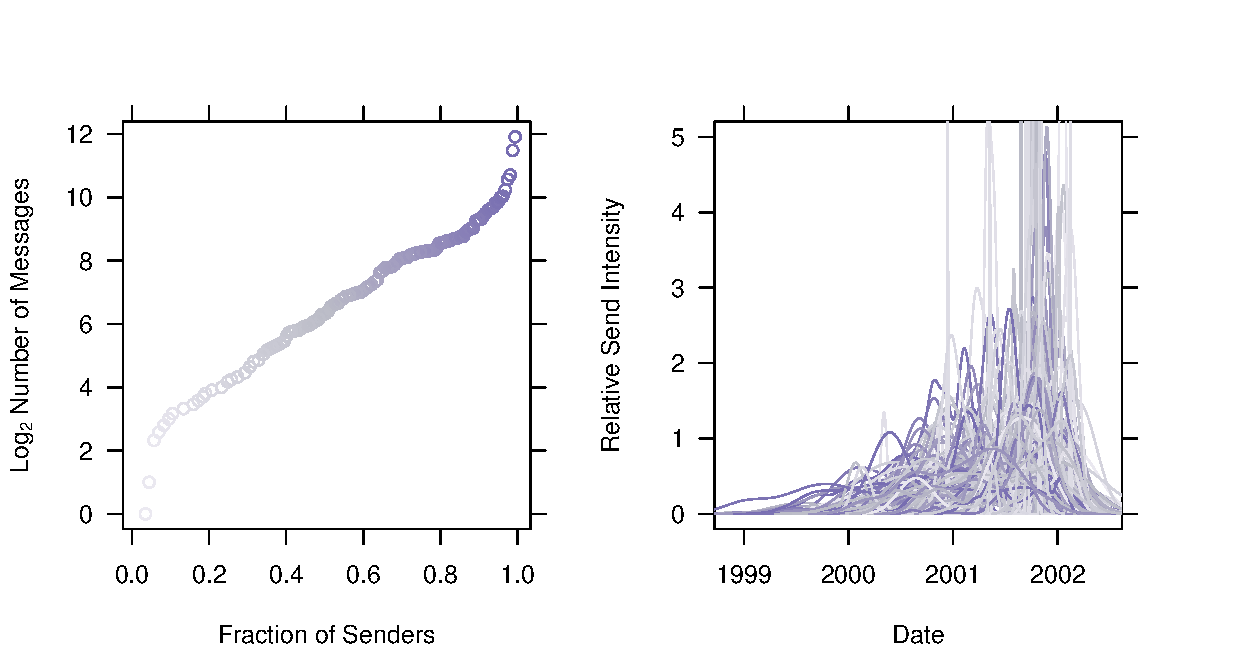
\includegraphics[scale=0.6]{figures/send-intensities}
    \caption{
        \textsc{Send intensities of all 156 employees in the Enron
        dataset.}  The curves in the right panel are constructed as in
        Fig.~\ref{F:kernel-intensity}, except normalized so that the
        area under each curve is one.   The left panel shows a quantile plot
        of the number of the normalization constants,
        the messages sent per sender (numbers range from 1 to 3,844).
        Colors are consistent across the two panels.
        The two panels reveal inhomogeneity of sending volumes and of
        activity behaviors.
    }
    \label{F:send-intensities}
\end{figure}
Malmgen et. al use a hidden Markov
model to capture individual and seasonal idiosyncrasies
\cite{malmgen2009characterizing}; we use a nonparametric model instead.

******

\section{A Point Process Model and Partial-Likelihood Inference}\label{S:point-process-model}

Every interaction process can be encoded by a multivariate counting measure.
For sender $i$, receiver $j$, and positive time $t$, define
\[
    N_t(i,j)
        =
        \#\{
            \text{directed interactions $i\rightarrow j$ in time interval 
            $[0,t]$}
        \}.
\]
For technical reasons, assume $N_0(i,j) = 0$ and that $N_t(i,j)$ is adapted to 
a stochastic basis of $\sigma$-algebras $\{ \mathcal{F}_t \}_{t \geq 0}$
satisfying the usual  conditions.  Then, $N_t(i,j)$ is a 
local submartingale, so by the Doob-Meyer decomposition, there exists a 
predictable increasing process $\Lambda_t(i,j)$, null at zero, such that $N_t(i,j) - \Lambda_t(i,j)$ is an $\mathcal{F}_t$ local martingale.  Under mild conditions---the most important of which is that no two 
interactions happen simultaneously---there exists a predictable continuous 
process $\lambda_t(i,j)$ such that
\(
    \Lambda_t(i,j) = \int_0^t \lambda_s(i,j) \, ds.
\)
(In practical applications, simultaneous events exist and are an annoyance;
Efron be handles them through an ad-hoc adjustment, while Brostr\"om adds a 
discrete component to $\Lambda$ \cite{efron1977efficiency,brostrom2002cox}.)
The process $\lambda$ is known as the stochastic intensity of $N$.
Heuristically,
\[
    \lambda_t(i,j) \, dt
        =
        \mathbb{P}\{
            \text{interaction $i\rightarrow j$ occurs in time interval $[t,t+dt)$}
        \}.
\]
We will model $N$ through $\lambda$ using a version of the Cox
proportional intensity model \cite{cox1972regression}.  

Let $\mathcal{I}$ be a set of senders and $\mathcal{J}$ be a set of receivers.
For each sender $i$, let $\bar \lambda_t(i)$ be a non-negative predictable
process called the baseline intensity of sender $i$; let $\mathcal{J}_t(i)$ be 
a predictable subset of $\mathcal{J}$ called the receiver set of sender $i$.
For each sender-receiver pair $(i,j)$, let $x_t(i,j)$ be a predictable
locally bounded vector of covariates in $\reals^p$.  Let $\beta_0$
be an unknown vector of coefficients in  $\reals^p$.  For this section, 
assume each interaction has a single receiver.

Given a multivariate counting process $N$ on 
$\reals_+ \times \mathcal{I} \times \mathcal{J}$,
we model its stochastic intensity as
\begin{equation}\label{E:cox-intensity}
    \lambda_t(i,j)
        =
        \bar \lambda_t(i)
        \cdot
        \exp\{ \beta_0^\trans x_t(i, j) \}
        \cdot
        1{\{j \in \mathcal{J}_t(i)\}}.
\end{equation}
The model posits sender $i$ in $\mathcal{I}$ interacts  with receiver $j$ 
in $\mathcal{J}_t(i)$ at a baseline rate $\bar \lambda_t(i)$ modulated up or 
down according to the pair's covariate vector, $x_t(i,j)$.  As Efron notes
\cite{efron1977efficiency}, the specific parametric form for the multiplier
$\exp\{ \beta_0^\trans x_t(i,j) \}$ is not central to the theoretical 
analysis, but this form is amenable to computation and gives
the parameter vector $\beta_0$ a straightforward interpretation.

The form of \eqref{E:cox-intensity} is deceptively simple but remains 
flexible enough to be useful in practice.  Of course, the model allows for
homophily and group level effects via inclusion of covariates like
``$1\{\text{$i$ and $j$ belong to the same group}\}$,'' where ``group'' is 
some observable trait like ethnicity, gender, or age group.  The real strength
of the model is that $x_t(i,j)$ is allowed to be \emph{any} predictable
process, in particular it can depend on the history of interactions.  To
model reciprocation or transitivity in the interactions  (assuming 
$\mathcal{I} = \mathcal{J}$), choose a positive $\delta$ and include 
covariates in $x_t(i,j)$ like
\[
    1\{\text{interaction $j \to i$ occurred in $[t - \delta,t)$}\}
\]
or
\[
    1\{\text{for some $k$, interaction $i\to k$ and $k \to j$ occurred in
             $[t - \delta, t)$}\}.
\]
Any process measurable with respect to the predictable $\sigma$-algebra is
a valid covariate; this only excludes covariates depending on the future
or the immediate present.

Following Cox \cite{cox1975partial}, we treat the baseline rate
$\bar \lambda_t(i)$ as a nuisance parameter estimate the coefficient
$\beta_0$ vector using a partial likelihood.  Let
$(t_1, i_1, j_1), \ldots, (t_n, i_n, j_n)$ be the sequence of observed
interactions.  Heuristically, partial likelihood is motivated by decomposing 
the likelihood as
\begin{align*}
    \begin{split}
    f(t_1&, i_1, j_1, t_2, i_2, j_2, \ldots, t_n, i_n, j_n) \\
        &=
            f(t_1, i_1)
            \, f(j_1 | t_1, i_1)
            \, f(t_2, i_2 | t_1, i_1, j_1)
            \, f(j_2 | t_2, i_2, t_1, i_1, j_1) \\
        &\quad \cdots
            f(t_n, i_n | t_{n-1}, i_{n-1}, j_{n-1}, \ldots t_1, i_1, j_1)
            \, f(j_n | t_{n-1}, i_{n-1} \ldots t_1, i_1, j_1)
    \end{split} \\
    \begin{split}
        &=
            \Big[
                f(t_1, i_1)
                \, f(t_2, i_2 | t_1, i_1, j_1)
                \cdots
                f(t_n, i_n | t_{n-1}, i_{n-1}, j_{n-1}, \ldots t_1, i_1, j_1)
            \Big] \\
        &\quad
            \cdot
            \Big[
                f(j_1 | t_1, i_1)
                \, f(j_2 | t_2, i_2, t_1, i_1, j_1)
                \cdots
                f(j_n | t_{n-1}, i_{n-1} \ldots t_1, i_1, j_1)
            \Big];
    \end{split}
\end{align*}
the latter term is dubbed a partial likelihood.  In continuous time, the
the log partial likelihood at time $t$, evaluated at $\beta$, is
\begin{equation}\label{E:log-pl}
    \log
    \mathit{PL}_t(\beta)
        =
        \sum_{t_m \leq t}
        \bigg\{
            \beta^\trans x_{t_m}\!(i_m, j_m)
            -
            \log\big[
                \!\!\!\!
                \sum_{j \in \mathcal{J}_{t_m}\!(i_m)}
                    \exp\{ \beta^\trans x_{t_m}\!(i_m, j)\}
            \big]
        \bigg\}.
\end{equation}
In Section~\ref{S:MPLE-consistency} we prove under suitable regularity
conditions that the maximizer of $\log \mathit{PL}_t(\cdot)$ is a
consistent estimator of $\beta_0$ as $t$ increases.

Function $\log \mathit{PL}_t(\cdot)$ is concave, and so can be maximized
via Newton's method or a gradient-based optimization method
\cite{nocedal2006numerical}.  These methods require one or both of the
first two derivatives of $\log\mathit{PL}_t(\cdot)$, which can be
expressed as weighted mean and covariance of the covariates.  The weights are
\begin{subequations}
\begin{align}
    w_{t}(\beta, i,j)
        &=
        \exp\{ \beta^\trans x_t(i,j) \}
        \cdot
        1\{ j \in \mathcal{J}_t(i)\}, \\
    \text{and}\qquad
    W_{t}(\beta, i)
        &=
        \sum_{j \in \mathcal{J}} w_{t}(\beta, i,j).
\end{align}
\end{subequations}
The inner sum in $\log \mathit{PL}_t(\beta)$ is
$W_{t_m}\!(\beta, i_m)$.  The function
$\log W_{t}(\cdot, i)$ has gradient $E_{t}(\cdot, i)$ and Hessian
$V_{t}(\cdot, i)$, given by
\begin{subequations}
\begin{gather}
    E_{t}(\beta, i)
        =
        \frac{1}{W_{t}(\beta, i)}
        \sum_{j \in \mathcal{J}_t(i)}
            w_{t}(\beta, i,j) \, x_{t}(i,j), \label{E:wt-expectation}\\
    V_{t}(\beta, i)
        =
        \frac{1}{W_{t}(\beta, i)}
        \sum_{j \in \mathcal{J}_t(i)}
            w_{t}(\beta, i,j)
            \Big[ x_{t}(i,j) - E_{t}(\beta, i)\Big]^{\otimes 2},
\end{gather}
\end{subequations}
where $a^{\otimes 2} = a \otimes a = a a^\trans$.
Consequently, the gradient and negative Hessian of
$\log \mathit{PL}_t(\cdot)$ are
\begin{subequations}
\begin{gather}
    \label{E:log-pl-gradient}
    U_t(\beta)
        =
        \nabla \big[ \log \mathit{PL}_t(\beta) \big]
        =
        \sum_{t_m \leq t}
            x_{t_m}(i_m, j_m) - E_{t_m}(\beta, i_m), \\
    \label{E:log-pl-neg-hessian}
    I_t(\beta)
        =
        -\nabla^2 \big[ \log \mathit{PL}_t(\beta) \big]
        =
        \sum_{t_m \leq t}
            V_{t_m}(\beta, i_m).
\end{gather}
\end{subequations}
We call $U_t(\beta_0)$ the unnormalized score and $I_t(\beta_0)$
the Fisher information matrix.

\section{Consistency of Maximum Partial Likelihood Inference}
\label{S:MPLE-consistency}

Under the model of Section~\ref{S:point-process-model}, the maximum partial likelihood estimator (MPLE) is a natural
estimate of $\beta_0$; the inverse Hessian of $\log \mathit{PL}_t(\cdot)$
evaluated at the MPLE is a natural estimate of its covariance matrix.
We now give conditions under which these
estimators are consistent as $t$ goes to infinity.

In the sampling regime where observation time $t$ is fixed and the number of 
senders $|\mathcal{I}|$ increases, Anderson and Gill's consistency proof for
the Cox proportional hazards model in survival analysis extends
to cover model~\eqref{E:cox-intensity}.  This setting is natural in the 
context of clinical trial data, where $\mathcal{I}$ corresponds to the set of 
patients under study, but does not meet the requirements typical of 
interaction data.  For most interaction 
data we cannot control $\mathcal{I}$ and $\mathcal{J}$, and the only way to 
get more data is to increase $t$.  Cox gives a rough proof for general
MPLE consistency which applies to our sampling regime but his argument is 
heuristic; Wong's treatment is more rigorous but does not cover continuous or 
time-varying covariates \cite{cox1975partial,wong1986theory}. The general 
interaction data sampling regime mandates a new consistency proof.

Despite assuming $\mathcal{I}$ and $\mathcal{J}$ to be effects, our analysis 
allows senders and receivers to enter and leave the study during the 
observation period.  The effective number of senders at time $t$ is the
set of $i$ such that $\bar \lambda_t(i) \neq 0$, which potentially varies
with time.  Likewise, the effective number of receivers is controlled through
$\mathcal{J}_t(i)$.

Our consistency proof relies on rescaling time to make the interaction 
times uniform.  To this end, define marginal processes
\(
    N_t(i) = \sum_{j \in \mathcal{J}} N_t(i,j)
\)
and
\(
    N_t = \sum_{i \in \mathcal{I}} N_t(i),
\)
define sequence of stopping times
\begin{equation}\label{E:message-times}
    \tau_n = \sup\{ t : N_t < n \},
\end{equation}
and let $\mathcal{F}_{\tau_n}$ be the $\sigma$-algebra of events prior to
$\tau_n$. The main idea of the proof is to change time from the original scale 
to a scale on which $\tau_{n} - \tau_{n'}$ is proportional to $n - n'$.

\subsection{Assumptions}

Let $\mathcal{B}$ be a neighborhood of $\beta_0$.  For a vector, $a$, let
$\| a \|$ denote its Euclidean norm; for a matrix, $A$, let $\| A \|$ denote
its spectral norm (largest eigenvalue).  We require the following assumptions:
\begin{enumerate}[{A}1.]
    \item \label{A:square-int}
    \textbf{The covariates are uniformly square-integrable.}  That is,
    \[
        \E\left[
            \sup_{t, i, j} \| x_{t}(i,j) \|^2
        \right]
        \,\,\text{is bounded.}
    \]

    \item \label{A:integrated-cov-limit}
    \textbf{The integrated covariance function is well-behaved.}
    When $\beta \in \mathcal{B}$ and $\alpha \in [0,1]$, as $ n \to \infty$,
    \[
        \frac{1}{n}
        \sum_{i \in \mathcal{I}}
        \int_0^{\tau_{\lfloor \alpha n \rfloor}}
            V_s(\beta,i)
            \, W_s(\beta,i)
            \, \bar \lambda_s(i)
            \, ds
        \toP
        \Sigma_\alpha(\beta).
    \]

    \item \label{A:message-times-finite}
    \textbf{The interaction arrival times are finite.}  For each $n$,
    \[
        \mathbb{P}\{\tau_n < \infty\} = 1.
    \]

    \item \label{A:var-equicont}
    \textbf{The variance function is equicontinuous.}
    More precisely,
    \[
        \Big\{
            V_{\tau_n}(\cdot, i)
            :
            n \geq 1, i \in \mathcal{I}
        \Big\}
        \,\,\text{is an equicontinuous family of functions.}
    \]
\end{enumerate}

These technical assumptions are similar to those of Anderson and 
Gill~\cite{andersen1982cox}, who investigate specific settings in which their 
assumptions hold.  Under A\ref{A:message-times-finite} the other three 
assumptions hold when $\| x_t(i,j) \|$ is bounded.

\subsection{Main Results}
Assumptions A\ref{A:square-int}--A\ref{A:var-equicont} imply that the MPLE is consistent and asymptotically
Gaussian, as shown by the following two theorems.  
%Their proofs follow immediately, with technical lemmas deferred to Appendix~\ref{S:MPLE-consistency-proofs}.

\begin{theorem}\label{T:score-fisher}
    Let $N$ be a multivariate counting process with stochastic
    intensity as given in~\eqref{E:cox-intensity}, with true parameter
    vector $\beta_0$.  Let $\tau_n$ be the sequence of message arrival times
    defined in~\eqref{E:message-times}, set $U_t(\beta)$ and $I_t(\beta)$ to
    be the gradient and negative Hessian of the log partial likelihood function
    as given in~(\ref{E:log-pl-gradient}--\ref{E:log-pl-neg-hessian}).  If
    assumptions A\ref{A:square-int}--A\ref{A:integrated-cov-limit} hold, then
    as $n \to \infty$:
    \begin{enumerate}[(i)]
        \item \label{I:score-part}
        $n^{-1/2} \, U_{\tau_{\lfloor \alpha n \rfloor}}(\beta_0)$
        converges weakly to a Gaussian process on $[0,1]$ with
        covariance function $\Sigma_\alpha(\beta_0)$;

        \item \label{I:fisher-part}
        if assumptions
        A\ref{A:message-times-finite}--A\ref{A:var-equicont} also hold, then for any consistent
        estimator $\hat \beta_n$ of $\beta_0$,
        we have that
        \[
            \sup_{\alpha \in [0,1]}
            \left\|
                \tfrac{1}{n}
                I_{\tau_{\lfloor \alpha n \rfloor}}(\hat \beta_{n})
                -
                \Sigma_\alpha(\beta_0)
            \right\|
            \toP
            0.
        \]
    \end{enumerate}
\end{theorem}

\noindent
We don't actually require convergence of the whole sample path, but
it turns out to be just as much effort to prove as convergence of the
endpoint.  

Consistency is a direct consequence of Theorem~\ref{T:score-fisher}
(Appendix~\ref{S:MPLE-consistency-proofs} contains a proof).

\begin{theorem}\label{T:consistency}
    Let $N$ be a multivariate counting process on with stochastic
    intensity as given in~\eqref{E:cox-intensity}, with true parameter
    vector $\beta_0$.  Let the log partial likelihood,
    $\log \mathit{PL}_t(\cdot)$, be as defined in \eqref{E:log-pl}.
    Let $\tau_n$ be the sequence of message arrival times defined
    in~\eqref{E:message-times}.

    Assume for $\beta$ in a
    neighborhood of $\beta_0$ that
    \(
        -\tfrac{1}{n} \nabla^2 [ \log \mathit{PL}_{\tau_n}(\beta)]
            \toP \Sigma_1(\beta),
    \)
    where $\Sigma_1(\cdot)$ is locally Lipschitz and with smallest eigenvalue bounded
    away from zero.
    If $\hat \beta_n$ maximizes $\log \mathit{PL}_{\tau_n}(\cdot)$ and
    conclusion~(\ref{I:score-part}) of Theorem~\ref{T:score-fisher} holds,
    then the following are true as $n\to\infty$:
    \begin{enumerate}[(i)]
        \item $\hat \beta_n$ is a consistent estimator of $\beta_0$;
        \item $\sqrt{n} \, (\hat \beta_n - \beta_0)$ converges weakly
            to a mean-zero Gaussian random variable with covariance
            $[\Sigma_1(\beta_0)]^{-1}$.
    \end{enumerate}
\end{theorem}

\begin{proof}[Proof of Theorem~\ref{T:score-fisher}]%, Part \textit{(\ref{I:score-part})}]
Observe that the process $N_t(i,j)$ has compensator
\(
    \Lambda_t(i,j)
        =
            \int_0^t \lambda_s(i,j) \, ds;
\)
similarly, processes $N_t(i)$ and $N_t$ have compensators
$\Lambda_t(i) = \sum_{j \in \mathcal{J}} \Lambda_t(i,j)$
and $\Lambda_t = \sum_{i \in \mathcal{I}} \Lambda_t(i)$.  Correspondingly, define local
martingales $M_t(i,j) = N_t(i,j) - \Lambda_t(i,j)$,
$M_t(i) = N_t(i) - \Lambda_t(i)$, and
$M_t = N_t - \Lambda_t$.
Define
\[
    H_t(i,j)
        =
        x_t(i,j) - E_t(\beta_0,i),
\]
where $E_t(\beta,i)$ is as defined in \eqref{E:wt-expectation}.

As observed by Andersen and Gill \cite{andersen1982cox}, the score function 
$U_t(\cdot)$ evaluated at $\beta_0$ has 
a simple representation in terms of these processes:
\begin{align*}
    U_t(\beta_0)
        &=
        \sum_{i \in \mathcal{I}}
        \sum_{j \in \mathcal{J}}
        \int_0^t
            H_s(i,j) \, dN_s(i,j) \\
        &=
        \sum_{i \in \mathcal{I}}
        \sum_{j \in \mathcal{J}}
        \int_0^t
            H_s(i,j) \, dM_s(i,j),
\end{align*}
since
\(
    \sum_{j \in \mathcal{J}}
    \int_0^t
        H_s(i,j) \,
        d\Lambda_s(i,j)
    =
    0.
\)
Since by Assumption A\ref{A:square-int}, $x$ is uniformly bounded, $H$ is as well.  Each term in the sum above is thus locally square integrable, with predictable covariation
\begin{align*}
    \begin{split}
        \bigg\langle
            \int
                H_s(i,j) \, dM_s(i,j)
        &, \, \,
            \int
                H_s(i',j') \, dM_s(i',j')
        \bigg\rangle_t \\
        &=
            \int_0^t
                H_s(i,j) \otimes H_s(i',j') \,
                d\big\langle M(i,j), M(i',j')\big\rangle_s
    \end{split} \\
        &=
            \int_0^t
                \big[ H_s(i,j) \big]^{\otimes 2} \,
                d\Lambda_s(i,j)
            \cdot
            1\{ i = i', j = j' \}
\end{align*}
\cite[Thm.~2.4.3]{fleming1991counting}.  There exists a sequence
of stopping times localizing all $M(i,j)$ simultaneously, so $U(\beta_0)$ is
locally square integrable with predictable variation
\begin{align}
\begin{split}\label{E:score-compensator}
    \big\langle U(\beta_0) \big\rangle_t
        &=
            \sum_{i \in \mathcal{I}}
            \sum_{j \in \mathcal{J}}
            \int_0^t
                \big[ H_s(i,j) \big]^{\otimes 2} \,
                d\Lambda_s(i,j) \\
        &=
            \sum_{i \in \mathcal{I}}
            \int_0^t
                V_s(\beta_0, i) \,
                d\Lambda_s(i).
\end{split}% \\
%\intertext{Note}\label{E:var-estimate}
%    I_t(\beta)
%        &=
%            \sum_{i \in \mathcal{I}}
%            \int_0^t
%                V_s(\beta, i) \,
%                dN_s(i).
\end{align}

Now we rescale time.  For each positive $n$ define a discretized time-scaled version of the score that is right-continuous with limits from the left.  The process is defined for times $\alpha$ in $[0,1]$; between times in $[\tfrac{k}{n}, \tfrac{k+1}{n})$, it takes the value $U_{\tau_k}$; i.e.,
\[
    \tilde U_{\alpha}^{(n)}(\beta)
        = U_{\tau_{\lfloor \alpha n \rfloor}}(\beta).
\]

Part~\textit{(\ref{I:score-part})}: 
Lemma~\ref{L:adapted-martingale} shows that $\tilde U_\alpha^{(n)}(\beta_0)$ is a square-integrable martingale
adapted to
\(
    \mathcal{\tilde F}^{(n)}_\alpha
        =
        \mathcal{F}_{\tau_{\lfloor \alpha n \rfloor}},
\)
the $\sigma$-algebra of events prior to
$\tau_{\lfloor \alpha n \rfloor}$.
Since it only depends on values at jump times, the
quadratic variation of $\tilde U^{(n)}(\beta_0)$ at time $\alpha$ is
equal to the quadratic variation of $U(\beta_0)$ at time
$\tau_{\lfloor \alpha n \rfloor}$.  Therefore, since quadratic and predictable
variation have the same limit when it exists
\cite[Prop.~1]{rebolledo1980central}, assumption A\ref{A:integrated-cov-limit}
implies that
\(
    \langle \frac{1}{\sqrt{n}} \tilde U^{(n)}(\beta_0) \rangle_\alpha
        \toP
            \Sigma_\alpha(\beta_0).
\)
Lemma~\ref{L:Lindeberg-condition} in turn verifies that $\frac{1}{\sqrt{n}} \tilde U^{(n)}(\beta_0)$ satisfies a Lindeberg condition necessary for the application of Rebolledo's Martingale Central Limit Theorem~\cite{rebolledo1980central}.  Thus the process converges in distribution to a Gaussian process with covariance function $\Sigma_\alpha(\beta_0)$ as claimed.

Part~\textit{(\ref{I:fisher-part})}:
Recalling $M_t(i) = N_t(i) - \Lambda_t(i)$, we may combine~\eqref{E:log-pl-neg-hessian} and~\eqref{E:score-compensator} to obtain the relation
\begin{equation}\label{E:var-estimate-relation}
            \sum_i
            \int_0^{\tau_{\lfloor \alpha n \rfloor}}
                V_s(\beta_0, i) \, dM_s(i)
        =
            I_{\tau_{\lfloor \alpha n \rfloor}}(\beta_0)
        -
            \big\langle \tilde U^{(n)}(\beta_0) \big\rangle_\alpha.
\end{equation}

When $\alpha \in [0, 1]$, then, a repeated application of the triangle inequality 
to 
\(
    \left\|
        \tfrac{1}{n} I_{\tau_{\lfloor \alpha n \rfloor}}(\hat \beta_n)
        -
        \tfrac{1}{n} \{ I_{\tau_{\lfloor \alpha n \rfloor}}(\beta_0) - I_{\tau_{\lfloor \alpha n \rfloor}}(\beta_0) \}
        -
        \Sigma_{\alpha} (\beta_0)
    \right\|
\)
using the relation~\eqref{E:var-estimate-relation} yields
\begin{align*}
    \left\|
        \tfrac{1}{n} I_{\tau_{\lfloor \alpha n \rfloor}}(\hat \beta_n)
        -
        \Sigma_{\alpha} (\beta_0)
    \right\|
        &\leq
        \left\|
            \frac{1}{n}
            \sum_i
            \int_0^{\tau_{\lfloor \alpha n \rfloor}}
                \{
                    V_s(\hat \beta_n, i)
                    -
                    V_s(\beta_0, i)
                \} \, dN_s(i)
        \right\| \\
        &\quad+
        \left\|
            \frac{1}{n}
            \sum_i
            \int_0^{\tau_{\lfloor \alpha n \rfloor}}
                V_s(\beta_0, i) \, dM_s(i)
        \right\| \\
        &\quad+
        \left\|
            \frac{1}{n}
            \sum_i
            \int_0^{\tau_{\lfloor \alpha n \rfloor}}
                V_s(\beta_0,i)
                \, d\Lambda_s(i)
            -
            \Sigma_{\alpha}(\beta_0)
        \right\|.
\end{align*}
The first term above is uniformly bounded by
\(
    \sup_{n',i}
        \|
            V_{\tau_{n'}}(\hat \beta_n, i)
            -
            V_{\tau_{n'}}(\beta_0, i)
        \|,
\)
which converges to zero since $\hat \beta_n \toP \beta_0$ by hypothesis of the theorem and
$\{ V_{\tau_{n'}}(\cdot, i) \}$ is an equicontinuous family by assumption~A\ref{A:var-equicont}.  Lemma~\ref{L:Lenglart} proves, as a consequence of assumption~A\ref{A:message-times-finite} and Lenglart's Inequality~\cite{lenglart1977relation}, that the second term converges to zero uniformly in $\alpha$.
The third term converges to zero by assumption~A\ref{A:integrated-cov-limit}, thereby concluding the proof.

\end{proof}


\section{Multicast Interactions}\label{S:multiple-receivers}

In Sections~\ref{S:point-process-model}~and~\ref{S:MPLE-consistency},
we have assumed each interaction involves a single sender and a single 
receiver.  The model and corresponding asymptotic theory are sufficient to 
cover strictly pairwise directed interactions (e.g. phone calls), but they
do not extend to interactions that can involve multiple receivers (e.g. e-mail 
messages).  We call an interaction involving a single sender and possibly 
multiple receivers a multicast interaction.  

In practice, multicast interactions usually get treated in an ad-hoc manner 
via duplication---for example, interaction $i \to \{ j_1, j_2, j_3 \}$ gets 
recorded as three separate pairwise interactions, $i \to j_1$, $i \to j_2$, 
and $i \to j_3$---giving rise to approximate likelihood and inference.
In this section we explore the implications of using this approximate
likelihood for our model.  In particular we show  the approximation is closely 
related to an extension of the model and that bias introduced by the 
approximation can be quantified and in certain cases corrected.

To this end, we introduce an extension of the model to the multicast setting.
Let $\mathcal{I}$, $\mathcal{J}$, $\mathcal{J}_t(i)$, $x_t(i,j)$,
and $\beta_0$ be as in Section~\ref{S:point-process-model}.  For each sender 
$i$ and positive integer $L$, let $\bar \lambda_t(i ; L)$ be a non-negative 
predictable process called the baseline $L$-receiver intensity of sender $i$
Let $(t_1, i_1, J_1), \ldots, (t_n, i_n, J_n)$ be the 
sequence of observed multicast interactions, with tuple $(t, i, J)$ indicating 
that at  time $t$ sender $i$ interacted with receiver set $J$.  For a set
$J$, let $|J|$ denote its cardinality.

Consider a model for multicast interactions where the rate of interaction
between sender $i$ and receiver set $J$ is
\begin{equation}\label{E:intensity-multiple}
    \lambda_t(i,J)
        =
        \bar \lambda_t(i ; |J|)
        \cdot
        \exp\Big\{
            \sum_{j \in J}
                \beta_0^\trans  x_t(i,j)
        \Big\}
        \cdot
        \prod_{j \in J}
        1\{ j \in \mathcal{J}_t(i) \}.
\end{equation}
The log partial likelihood at time $t$, evaluated at $\beta$, is
\begin{equation}\label{E:log-pl-multiple}
    \log
    \mathit{PL}_t(\beta)
        =
        \sum_{t_m \leq t}\!
        \bigg\{\!
            \sum_{j \in J_m}\!
                \beta^\trans x_{t_m}\!(i_m, j)
            -
            \log\big[
                \!\!\!\!
                \sum_{\substack{J \subseteq \mathcal{J}_{t_m}(i_m) \\
                               |J| = |J_m|}}\!\!\!\!\!\!\!
                    \exp\big\{
                        \sum_{j \in J}
                            \beta^\trans x_{t_m}\!(i_m, j)
                    \big\}
            \big]
        \bigg\}.
\end{equation}

Suppose instead of using the multicast model, we use duplication to get
pairwise interactions from the original multicast data.  If we use
model~\eqref{E:cox-intensity} for the pairwise data and ignore ties in
the interaction times, we get an approximate partial likelihood:
\begin{equation}\label{E:log-pl-multiple-approx}
    \log
    \widetilde{\mathit{PL}}_t(\beta)
        =\!
        \sum_{t_m \leq t}\!
        \bigg\{\!
            \sum_{j \in J_m}\!
                \beta^\trans x_{t_m}\!(i_m, j)
            -
            |J_m|
            \log\big[
                \!\!\!\!
                \sum_{j \in \mathcal{J}_{t_m}\!(i_m)}\!\!\!\!\!
                    \exp\{ \beta^\trans x_{t_m}\!(i_m, j)\}
            \big]
        \bigg\}.
\end{equation}

We claim $\log \widetilde{\mathit{PL}}_t(\beta)$ is an approximation of
$\log \mathit{PL}_t(\beta)$.  Heuristically, replacing the
sum over all sets of size $|J_m|$ with a sum over all multisets of size
$|J_m|$ allowing duplicate elements,
\begin{align*}
    \log\big[\!\!
        \sum_{\substack{J \subseteq \mathcal{J}_{t_m}(i_m) \\
              |J| = |J_m|}}\!\!\!
            \exp\big\{
                \sum_{j \in J}
                    \beta^\trans x_{t_m}\!(i_m, j)
            \big\}
    \big]
    &\approx
        \log\big[\!\!\!
            \sum_{j \in \mathcal{J}_{t_m}(i_m)}\!\!\!\!\!
                \exp\big\{
                    \beta^\trans x_{t_m}\!(i_m, j)
                \big\}
        \big]^{|J_m|} \\
    &=
        |J_m|
        \log\big[\!\!\!
            \sum_{j \in \mathcal{J}_{t_m}(i_m)}\!\!\!\!\!
                \exp\big\{
                    \beta^\trans x_{t_m}\!(i_m, j)
                \big\}
        \big].
\end{align*}
In this sense,
$\log \mathit{PL}_t(\beta) \approx \log \widetilde{\mathit{PL}}_t(\beta)$.
Section~\ref{S:approximation-error} makes this statement more precise,
and Section~\ref{S:approximation-bias} analyzes the bias introduced by the approximation

\subsection{Approximation Error}\label{S:approximation-error}
Introduce the receiver set growth sequence
\begin{equation}\label{E:growth-constant}
    G_n
        =
            \sum_{t_m \leq \tau_n}
                \frac{1\{|J_m| > 1\}}{|\mathcal{J}_{t_m}(i_m)|}.
\end{equation}
This sequence plays a critical role in bounded the error introduced by
replacing $\log \mathit{PL}$ with $\log \widetilde{\mathit{PL}}$.
Note when $|\mathcal{J}_{t_m}(i_m)|$ is constant $G_n$ has linear growth,
but when $|\mathcal{J}_{t_m}(i_m)|$ increases $G_n$ often has sublinear 
growth.  For example, the Cauchy-Schwartz inequality gives
\[
    G_n
        \leq
            \sqrt{n}
            \cdot
            \bigg[
                \sum_{t_m \leq \tau_n}
                    \frac{1\{|J_m| > 1\}}{|\mathcal{J}_{t_m}(i_m)|^2}
            \bigg]^{1/2},
\]
so if $|\mathcal{J}_{t_m}(i_m)| = \omega(\sqrt{m})$ then
$G_n = \Oh(\sqrt{n})$.  Theorem~\ref{T:log-pl-multiple-approx-error} bounds
the approximation error in terms of $G_n$.

\begin{theorem}\label{T:log-pl-multiple-approx-error}
    Let $(t_m, i_m, J_m)$ be a sequence of observations from a multivariate
    point processes with intensity as given in~\eqref{E:intensity-multiple}.
    Set $\tau_n = t_n$.  Assume
    \(
        \sup_t \| x_t (i,j) \|
    \)
    and
    \(
        \sup_m | J_m |
    \)
    are bounded in probability.
    If $\log \mathit{PL}$ and $\log \widetilde{\mathit{PL}}$ are as
    defined in
    \textnormal{(}\ref{E:log-pl-multiple}--\ref{E:log-pl-multiple-approx}\textnormal{)},
    and $G_n$ is as defined in \eqref{E:growth-constant},
    then for $\beta$ in a neighborhood of $\beta_0$,
    \[
        \Big\|
        \nabla [\log \mathit{PL}_{\tau_n}(\beta) ]
        -
        \nabla [\log \widetilde{\mathit{PL}}_{\tau_n}(\beta) ]
        \Big\|
            =
            \OhP(G_n),
    \]
    and
    \[
        \Big\|
        \nabla^2 [\log \mathit{PL}_{\tau_n}(\beta) ]
        -
        \nabla^2 [\log \widetilde{\mathit{PL}}_{\tau_n}(\beta) ]
        \Big\|
            =
            \OhP(G_n).
    \]
\end{theorem}

\begin{proof}[Proof of Theorem~\ref{T:log-pl-multiple-approx-error}]

When $J \subseteq \mathcal{J}_t(i)$, set
\(
    X_t(i, J) = \sum_{j \in J} x_t(i,j)
\)
and
\(
    w_t(\beta, i, J)
        = \exp\{ \beta^\trans X_t(i,J) \}.
\)
As a slight abuse of notation, when $j$ is an element of $\mathcal{J}_t(i)$,
take ``$w_t(\beta, i, j)$'' to mean $w_t(\beta, i, \{j\})$.  Define weights
\begin{subequations}
\begin{gather*}
    W_t(\beta, i; L)
        = \sum_{\substack{J \subseteq \mathcal{J}_t(i), \\
                          |J| = L}}
              w_t(\beta,i,J), \\
    \widetilde W_t(\beta, i; L)
        =
            \Big[ \sum_{j \in \mathcal{J}_t(i)} w_t(\beta, i, j) \Big]^L.
\end{gather*}
\end{subequations}
Approximation error in $\log \widetilde{\mathit{PL}}$ comes from replacing
$W$ with $\widetilde W$.

The gradients of the weights are
\begin{subequations}
\begin{gather*}
    E_t(\beta, i; L)
        = \nabla \big[ \log W_t(\beta, i; L) \big]
        =
        \frac{1}{W_t(\beta, i; L)}
        \sum_{\substack{J \subseteq \mathcal{J}_t(i), \\
                        |J| = L}}\!
            w_t(i,J)
            \,
            X_t(i,J), \\
    \widetilde E_t(\beta, i; L)
        = \nabla \big[ \log \widetilde W_t(\beta, i; L) \big]
        =
        L
        \cdot
        \frac{
            \sum_{j \in \mathcal{J}_t(i)}
                w_t(\beta, i, j) \, x_t(i,j)
        }{
            \sum_{j \in \mathcal{J}_t(i)}
                w_t(\beta, i, j)
        }.
\end{gather*}
\end{subequations}
The second is the expectation of $\sum_{l = 1}^L x_t(i, j_l)$ when
$j_1, \ldots, j_L$ are drawn independently and identically from
$\mathcal{J}_t(i)$ with weights $w_t(\beta, i, \cdot)$; the first is the same
expectation, conditional on the event that $j_1, \ldots, j_L$ are all unique.
Let $\tilde{\mathbb{P}}_{t,\beta,i;L}$ and $\mathbb{P}_{t,\beta,i;L}$
denote the two probability laws for $j_1, \ldots, j_L$, and let
$\tilde{\mathbb{E}}_{t,\beta,i;L}$ and $\mathbb{E}_{t,\beta,i;L}$ denote
expectations with respect to them, so that
$E_t(\beta,i;L) = \mathbb{E}_{t,\beta,i;L} \big[ \sum_{l=1}^L x_t(i,j_l)\big]$
and
\(
    \widetilde E_t(\beta,i;L)
    =
    \tilde{\mathbb{E}}_{t,\beta,i;L} \big[ \sum_{l=1}^L x_t(i,j_l)\big].
\)

The bound on 
\(
    \nabla [\log \mathit{PL}_{\tau_n}(\beta) ]
    -
    \nabla [\log \widetilde{\mathit{PL}}_{\tau_n}(\beta) ]
\)
derives from a bound on
\(
    E_t(\beta,i;L)
    -
    \widetilde E_t(\beta,i;L).
\)
Write
\[
    E_{t}(\beta, i; L) - \widetilde{E}_t(\beta, i; L)
        =
        \mathbb{E}_{t,\beta,i;L}
            \Big[ \sum_{l=1}^L x_t(i,j_l) \Big]
        -
        \widetilde{\mathbb{E}}_{t,\beta,i;L}
            \Big[ \sum_{l=1}^L x_t(i,j_l) \Big].
\]
We define probability law $\mathbb{P}^\ast_{t,\beta,i;L}$ and 
associated random variables $j_1, \ldots, j_L$ and
$\tilde \jmath_1, \ldots, \tilde \jmath_L$, such that marginally
$j_1, \ldots, j_L$ are distributed according to $\mathbb{P}_{t,\beta,i;L}$
and $\tilde \jmath_1, \ldots, \tilde \jmath_L$ are distributed according
to $\tilde{\mathbb{P}}_{t,\beta,i;L}$, but the variables are coupled to have
nontrivial chance of agreeing.  Then,
\begin{align*}
    \Big\| E_{t}(\beta, i; L) &- \widetilde{E}_t(\beta, i; L) \Big\| \\
        &=
            \Big\|
            \mathbb{E}_{t,\beta,i;L}^\ast
            \Big[
                \sum_{l=1}^L x_t(i,j_l)
                -
                \sum_{l=1}^L x_t(i, \tilde \jmath_l)
            \Big]
            \Big\| \\
        &\leq
            2 L
            \cdot
            \Big[
                \sup_{j \in \mathcal{J}_t(i)}
                \| x_t(i,j) \|
            \Big]
            \cdot
            \mathbb{P}^\ast_{t,\beta,i;L}
            \Big\{
                (j_1, \ldots, j_L)
                    \neq
                    (\tilde \jmath_1, \ldots, \tilde \jmath_L)
            \Big\}
\end{align*}
The coupling is as follows:
\begin{enumerate}
    \item Draw $(\tilde \jmath_1, \ldots, \tilde \jmath_L)$ according to
        $\tilde{\mathbb{P}}_{t,\beta,i;L}$.
    \item If $(\tilde \jmath_1, \ldots, \tilde \jmath_L)$ are all unique,
        set $(j_1, \ldots, j_L) = (\tilde \jmath_1, \ldots, \tilde \jmath_L)$,
        otherwise draw $(j_1, \ldots, j_L)$ independently according to
        $\mathbb{P}_{t,\beta,i;L}$.
\end{enumerate}
With $K = \sup_{j \in \mathcal{J}_t(i)} \| x_t(i,j) \|$, 
Lemma~\ref{L:coupling-prob-bound} shows
\[
    \mathbb{P}^\ast_{t,\beta,i;L}
    \Big\{
        (j_1, \ldots, j_L)
            \neq
            (\tilde \jmath_1, \ldots, \tilde \jmath_L)
    \Big\}
        \leq
        {L \choose 2}
        \cdot
        \frac{\exp\{4 K \, \| \beta \|\}}{| \mathcal{J}_t(i) |}.
\]
The resulting bound on 
\(
    \|
    \nabla [\log \mathit{PL}_{t}(\beta) ]
    -
    \nabla [\log \widetilde{\mathit{PL}}_{t}(\beta) ]
    \|
\)
now follows by expressing
\[
    \nabla \big[ \log \widetilde{\mathit{PL}}_t(\beta) \big]
    -
    \nabla \big[ \log \mathit{PL}_t(\beta )\big]
        =
        \sum_{t_m \leq t}
            E_{t_m}\!(\beta, i_m; |J_m|)
            -
            \widetilde{E}_{t_m}\!(\beta, i_m; |J_m|).
\]
Using
\(
    \big\| E_{t}(\beta, i; L) - \widetilde{E}_t(\beta, i; L) \big\|
        \leq
        K \, L^2 \, (L - 1)
        \,
        \frac{\exp\{4 K \, \| \beta \|\}}{| \mathcal{J}_t(i) |},
\)
we get
\[
    \Big\|
        \nabla\big[ \log \widetilde{\mathit{PL}}_t( \beta ) \big]
        -
        \nabla\big[ \log {\mathit{PL}}_t( \beta ) \big]
    \Big\| \\
        \leq
            K
            \exp\{4 K \| \beta \|\}
            \cdot
            \sum_{t_m \leq t}
                \frac{|J_m|^2(|J_m| - 1)}{|\mathcal{J}_{t_m}(i_m)|}.
\]
We get the final bound for the gradients by replacing the numerators of the 
summands with $\sup_m |J_m|$.

Using the same methods, Lemma~\ref{L:hessian-approx-bound} derives the bound 
on the difference in Hessians.
\end{proof}

\subsection{Bias Correction from the Approximate Partial Likelihood}
\label{S:approximation-bias}

When we use ad-hoc duplication, we are performing approximate inference
under the multicast model.  In practice, even if we explicitly want to use the
multicast model, computing the partial likelihood in \eqref{E:log-pl-multiple} 
involves an intractable combinatorial sum, so we may result to using the
approximation instead.  Maximizing $\log \widetilde{\mathit{PL}}_t(\cdot)$ 
instead of $\log \mathit{PL}_t(\cdot)$ introduces bias in the estimate of 
$\beta_0$.  Theorem~\ref{T:mple-approx-error} (proved in Appendix~\ref{S:multiple-recipient-proofs}) bounds the bias.

\begin{theorem}\label{T:mple-approx-error}
    Assume the setup of Theorem~\ref{T:log-pl-multiple-approx-error}.
    Let $\hat \beta_n$ maximize $\log \mathit{PL}_{\tau_n}(\cdot)$
    and let $\tilde \beta_n$ maximize
    $\log \widetilde{\mathit{PL}}_{\tau_n}(\cdot)$.
    Suppose for all $n$ that the norm of the Hessian,
    \(
        \|
        \tfrac{1}{n}
        \nabla^2
        [ \log \mathit{PL}_{\tau_n}(\cdot)]
        \|,
    \)
    is uniformly locally Lipschitz and bounded away from zero
    in a neighborhood of $\hat \beta_n$.
    If $G_n/n \toP 0$, then
    \[
        \| \tilde \beta_{n} - \hat \beta_{n} \|
            =
            \OhP(G_n/n).
    \]
\end{theorem}

It remains to be shown that $\hat \beta_n$ is a consistent estimator of
$\beta_0$.  This follows from the theory in Section~\ref{S:MPLE-consistency} 
since the multicast case can be considered as a special case of
the single receiver case.  The product $\mathcal{I} \times \mathbb{N}_+$
is the sender set and the power set $\mathcal{P}(\mathcal{J})$ is the
receiver set.  For sender $(i,L)$, the process $\bar \lambda(i ; L)$ is the
baseline send intensity and $\{ J \subseteq \mathcal{J}_t(i) : |J| = L\}$ is the receiver set; for
sender-receiver pair $\big((i,L), J\big)$, vector $\sum_{j \in J} x_t(i,j)$ is
the covariate vector.  Consistency of the MPLE now follows from
Theorem~\ref{T:consistency}.



Suppose the true MPLE, $\hat \beta_n$, is a $\sqrt{n}$-consistent estimate of
$\beta_0$ (Theorem~\ref{T:consistency} gives sufficient conditions).
Theorem~\ref{T:mple-approx-error} says that if
$|\mathcal{J}_{t_m}(i_m)|$ grows fast enough to make $G_n$ smaller than
$\OhP(\sqrt{n})$, then the approximate MPLE, $\tilde \beta_n$ is \emph{also}
$\sqrt{n}$-consistent.
Moreover, if $\sqrt{n}(\hat \beta_n - \beta_0)$ is asymptotically Gaussian,
then $\sqrt{n}(\tilde \beta_n - \beta_0)$ is asymptotically Gaussian with
the same covariance matrix but possibly a different mean.
Under enough regularity,
\(
    -\tfrac{1}{n} [
        \nabla^2 \log \widetilde{\mathit{PL}}_{\tau_n}(\tilde \beta_n)
    ]
\)
consistently estimates the limiting covariance
of $\sqrt{n}(\tilde \beta_n - \beta_0)$.  To get the mean, we use
a parametric bootstrap.

Assume the conditions of Theorem~\ref{T:mple-approx-error}.
The residual $\tilde \beta_n - \beta_0$ depends continuously on $\beta_0$
and the covariates, $x_t(i,j)$.  Since $\tilde \beta_n$ is a consistent
estimator of $\beta_0$, we can estimate the bias in $\tilde \beta_n$ via
a parametric bootstrap.  We generate a bootstrap replicate dataset
$\{ (t_m, i_m, J_m^{(r)}) \}$ by drawing $J_m^{(r)}$, a random subset
of $\mathcal{J}_{t_m}(i_m)$ with size $|J_m|$ whose elements are drawn
proportional to $w_{t_m}(\tilde \beta, i_m, \cdot)$.
We then get a bootstrap approximate MPLE, $\tilde \beta^{(r)}$, by maximizing
$\widetilde{\mathit{PL}}_{t_n}^{(r)}$, where
\begin{multline*}
    \log \widetilde{\mathit{PL}}_{t}^{(r)}\!(\beta) \\
        =
        \sum_{t_m \leq t}
        \bigg\{
            \sum_{j \in J_m^{(r)}}\!
                \beta^\trans x_{t_m}\!(i_m, j)
            -
            \log\big[
                \!\!\!\!
                \sum_{j \in \mathcal{J}_{t_m}\!(i_m)}
                    \exp\{ \beta^\trans x_{t_m}\!(i_m, j)\}
            \big]^{|J_m^{(r)}|}
        \bigg\}.
\end{multline*}
Note that $x_t(i,j)$ is determined from the original dataset, not the
bootstrap dataset.  For each bootstrap replicate, we get a residual
$\tilde \beta_n^{(r)} - \tilde \beta_n$.  With $R$ bootstrap
replicates, we estimate the bias by
\[
    \widehat{\mathrm{bias}}
        =
            \frac{1}{R} \sum_{r=1}^{R} \tilde \beta_n^{(r)} - \tilde \beta_n.
\]
We adjust for the bias by replacing $\tilde \beta_n$ with
$\tilde \beta_n - \widehat{\mathrm{bias}}$.


\begin{figure}
    %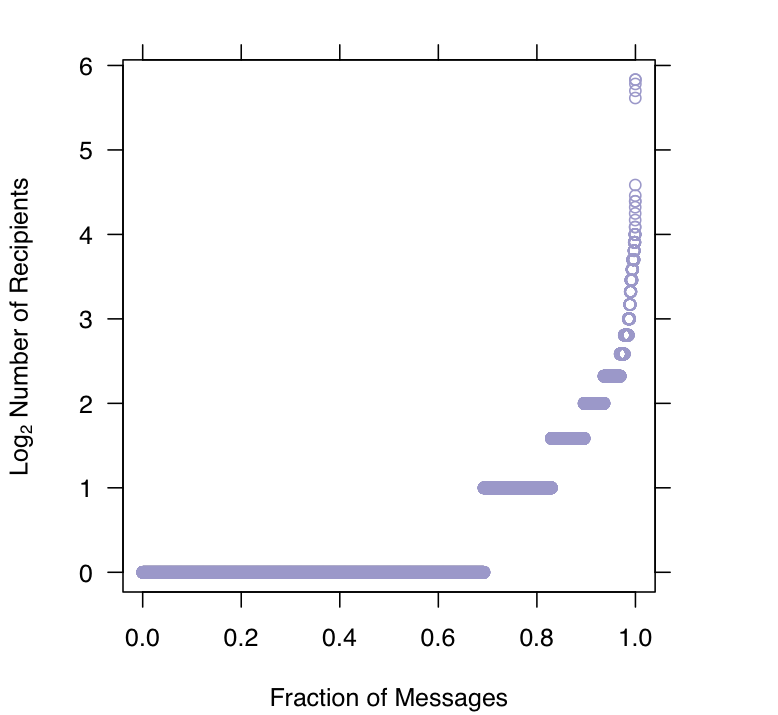
\includegraphics[scale=0.6]{figures/recipient-counts}
    \caption{
        \textsc{Message recipient counts.}
        Each of the 21,635 points corresponds to a message, with the
        $y$-value equal to the log (base 2) of the number of recipients
        for that message.  The message sent to the most people
        had 57 recipients.  In our analysis, we exclude messages with more
        than 10 recipients.
    }\label{F:recipient-counts}
\end{figure}



\section{Modeling the Enron Data}\label{S:enron-modeling}
% Retitle: Data Analysis?

****

 In the Enron dataset,
approximately 30\% of messages have more than one recipient, with
a few messages having more than fifty recipients
(see Fig.~\ref{F:recipient-counts}).  

****

For the data example we now consider,
the covariates are bounded and the message count is high, so
assumptions A\ref{A:square-int}--A\ref{A:var-equicont} and
the asymptotic framework are natural.

****

, and Appendix~\ref{S:implementaiton} presents
an efficient algorithm for computing them.  In practice, the
Hessian of $\log \mathit{PL}_t(\cdot)$ may be singular; when this is
the case, we introduce linear constraints on the parameters to make
them identifiable.

*****


*****

    In other e-mail datasets, people
    do sometimes e-mail themselves, but arguably these messages should be
    handled differently then messages exchanged between different individuals.

*****

Our motivating example is to test for gender bias in a corporate e-mail
network.  The dataset we use is a large collection of e-mail messages sent
within the Enron corporation during the last four years of the company's
existence.  Appendix~\ref{S:enron-corpus} describes the data collection and
preprocessing.  Briefly, there are 21,635 messages in the dataset, which
were sent between 156 executives in the company.  We know the genders,
seniorities, and departments of the employees (summarized in
Table~\ref{T:employee-summary}).

\begin{table}[h]
    
\begin{tabular}{lrclrclr}
    \toprule
    \multicolumn{2}{c}{\textbf{Gender}}
    & & \multicolumn{2}{c}{\textbf{Seniority}}
    & & \multicolumn{2}{c}{\textbf{Department}} \\
    \cmidrule{1-2} \cmidrule{4-5} \cmidrule{7-8}
    Female&43&&Junior&82&&Legal&25\\
    Male&113&&Senior&74&&Trading&60\\
    &&&&&&Other&71\\
    \bottomrule
\end{tabular}

    \caption{
        Characteristics of the 156 employees in the Enron dataset.
    }
    \label{T:employee-summary}
\end{table}

*****

To model the Enron data, we use the proportional intensity model with multiple
recipients from Section~\ref{S:multiple-recipients}.  Our analysis excludes
messages with more than 10 recipients---a
subjectively-chosen cutoff that includes 99\% of the corpus---because many of
these are ``broadcast'' and we are only interested in inter-personal
communication.  We fit the model by maximizing the approximate log partial
likelihood from \eqref{E:log-pl-multiple-approx}, and then apply
a bias-correction to be described in Section~\ref{S:bias-correction}.  For standard
errors, we use the forthcoming asymptotic theory and employ the delta method where
appropriate.

The senders and receivers are the 156 employees in the dataset, so
$\mathcal{I} = \mathcal{J} = \{ 1, 2, \ldots, 156 \}$.  To disallow
self-loops, we set $\mathcal{J}_t(i) = \mathcal{I} \setminus \{ i \}$.
We use two types of covariates: static and dynamic.  The static covariates
don't change over time, and are determined by the sender- and
receiver-specific group memberships summarized in
Table~\ref{T:employee-summary}.  The dynamic covariates depend on the
history of the process, and are chosen to allow adjusting for reciprocation
effects.  The next few paragraphs discuss the covariates in detail.

Considering gender (2 levels), seniority (2 levels), and department
(3 levels), each individual belongs to one of 12 groups.  Each
sender-receiver pair involves 2 of these groups, for $12^2 = 144$ possible
group-group combinations.  We introduce a static binary covariate for each
combination.  The dyad covariate vector $x_t(i,j)$ has 144 components
corresponding to these covariates.  For concreteness, abbreviate the codes
for gender, department, and seniority by F/M, L/T/O, and J/S.  For
individual $i$, define $s(i)$ in $\reals^{12}$ by
\begin{align*}
    s(i)
    =
    \big(
        &\text{1\{$i$ is FLJ\}},
        \text{1\{$i$ is FLS\}},
        \text{1\{$i$ is FTJ\}},
        \text{1\{$i$ is FTS\}}, \\
        &\,\,\text{1\{$i$ is FOJ\}},
        \text{1\{$i$ is FOS\}},
        \text{1\{$i$ is MLJ\}},
        \text{1\{$i$ is MLS\}}, \\
        &\,\,\,\,\text{1\{$i$ is MTJ\}},
        \text{1\{$i$ is MTS\}},
        \text{1\{$i$ is MOJ\}},
        \text{1\{$i$ is MOS\}}
    \big).
\end{align*}
The 144 static covariates of $x_t(i,j)$ are the interactions,
the components of $\vecm\big(s(i) \otimes s(j)\big)$, where
$a \otimes b = a b^\trans$ and $\vecm(\cdot)$ maps a matrix to a vector
by stacking columns.


\begin{table}[h]
    \tiny
    
\begin{tabular}{ll@{\,\,\,}rl@{\,\,\,}rl@{\,\,\,}rl@{\,\,\,}rl@{\,\,\,}rl@{\,\,\,}r}
\toprule
    & \multicolumn{12}{c}{\textbf{Sender}} \\
    \cmidrule(lr){2- 13 }
\textbf{Receiver}
    & \multicolumn{2}{c}{\textnormal{FLJ}}
    & \multicolumn{2}{c}{\textnormal{FLS}}
    & \multicolumn{2}{c}{\textnormal{FTJ}}
    & \multicolumn{2}{c}{\textnormal{FTS}}
    & \multicolumn{2}{c}{\textnormal{FOJ}}
    & \multicolumn{2}{c}{\textnormal{FOS}} \\
    \cmidrule(lr){1-1}
    \cmidrule(lr){2-3}
    \cmidrule(lr){4-5}
    \cmidrule(lr){6-7}
    \cmidrule(lr){8-9}
    \cmidrule(lr){10-11}
    \cmidrule(lr){12-13}
    \textnormal{FLJ} & \textbf{3.31} & (0.11) & 3.06 & (0.25) & 1.55 & (0.30) & 1.25 & (0.35) & 0.29 & (0.08) & 0.69 & (0.10) \\
    \textnormal{FLS} & 2.55 & (0.11) & 4.21 & (0.41) & 0.15 & (0.14) & 0.76 & (0.37) & 0.39 & (0.15) & 1.00 & (0.20) \\
    \textnormal{FTJ} & 0.43 & (0.06) & 0.61 & (0.24) & 1.36 & (0.33) & 1.39 & (0.38) & 0.46 & (0.12) & 1.00 & (0.29) \\
    \textnormal{FTS} & 0.81 & (0.12) & 0.49 & (0.14) & \textbf{4.34} & (1.11) & \textbf{2.53} & (0.65) & 2.22 & (0.28) & 0.19 & (0.10) \\
    \textnormal{FOJ} & 0.47 & (0.05) & 0.14 & (0.06) & 0.96 & (0.29) & 1.54 & (0.27) & \textbf{2.86} & (0.23) & 1.92 & (0.18) \\
    \textnormal{FOS} & 0.99 & (0.07) & 1.11 & (0.19) & 0.11 & (0.09) & 0.70 & (0.34) & 1.46 & (0.16) & \textbf{3.84} & (0.30) \\
    \textnormal{MLJ} & 1.41 & (0.10) & 1.03 & (0.28) & 3.62 & (0.69) & 0.65 & (0.42) & 1.48 & (0.32) & 0.76 & (0.15) \\
    \textnormal{MLS} & 3.07 & (0.11) & \textbf{4.48} & (0.35) & 1.15 & (0.45) & 0.65 & (0.21) & 0.35 & (0.09) & 1.48 & (0.14) \\
    \textnormal{MTJ} & 0.70 & (0.06) & 1.42 & (0.18) & 2.10 & (0.38) & 0.61 & (0.17) & 0.66 & (0.10) & 0.33 & (0.08) \\
    \textnormal{MTS} & 0.61 & (0.05) & 1.32 & (0.15) & 2.68 & (0.41) & 2.16 & (0.29) & 1.58 & (0.14) & 0.99 & (0.10) \\
    \textnormal{MOJ} & 0.47 & (0.04) & 0.27 & (0.05) & 2.16 & (0.35) & 1.34 & (0.21) & 1.62 & (0.13) & 0.75 & (0.08) \\
    \textnormal{MOS} & 0.86 & (0.06) & 0.71 & (0.10) & 0.13 & (0.10) & 0.37 & (0.14) & 2.39 & (0.20) & 3.74 & (0.28) \\
\end{tabular}

\begin{tabular}{ll@{\,\,\,}rl@{\,\,\,}rl@{\,\,\,}rl@{\,\,\,}rl@{\,\,\,}rl@{\,\,\,}r}
\phantom{\textbf{Receiver}} &\\
    & \multicolumn{2}{c}{\textnormal{MLJ}}
    & \multicolumn{2}{c}{\textnormal{MLS}}
    & \multicolumn{2}{c}{\textnormal{MTJ}}
    & \multicolumn{2}{c}{\textnormal{MTS}}
    & \multicolumn{2}{c}{\textnormal{MOJ}}
    & \multicolumn{2}{c}{\textnormal{MOS}} \\
    \cmidrule(lr){2-3}
    \cmidrule(lr){4-5}
    \cmidrule(lr){6-7}
    \cmidrule(lr){8-9}
    \cmidrule(lr){10-11}
    \cmidrule(lr){12-13}
    \textnormal{FLJ} & 2.21 & (0.24) & 2.97 & (0.24) & 0.27 & (0.07) & 0.08 & (0.02) & 0.14 & (0.06) & 0.70 & (0.12) \\
    \textnormal{FLS} & 0.45 & (0.24) & 2.46 & (0.21) & 2.33 & (0.35) & 0.42 & (0.08) & 0.11 & (0.07) & 0.38 & (0.09) \\
    \textnormal{FTJ} & 2.14 & (0.32) & 0.06 & (0.05) & \textbf{6.19} & (0.56) & \textbf{2.26} & (0.17) & 3.13 & (0.35) & 0.06 & (0.05) \\
    \textnormal{FTS} & 0.44 & (0.21) & 0.48 & (0.10) & 1.18 & (0.24) & 2.00 & (0.17) & 0.51 & (0.10) & 0.39 & (0.15) \\
    \textnormal{FOJ} & 0.39 & (0.10) & 0.26 & (0.06) & 0.27 & (0.07) & 1.01 & (0.09) & 2.07 & (0.19) & 3.32 & (0.35) \\
    \textnormal{FOS} & 1.80 & (0.30) & 2.35 & (0.21) & 0.13 & (0.06) & 1.68 & (0.14) & 2.13 & (0.26) & 2.24 & (0.22) \\
    \textnormal{MLJ} & 0.94 & (0.26) & 1.52 & (0.22) & 0.70 & (0.20) & 2.24 & (0.20) & 1.04 & (0.28) & 2.26 & (0.41) \\
    \textnormal{MLS} & 1.79 & (0.22) & \textbf{6.69} & (0.51) & 0.51 & (0.12) & 0.76 & (0.07) & 0.31 & (0.09) & 2.13 & (0.21) \\
    \textnormal{MTJ} & 0.67 & (0.14) & 1.33 & (0.14) & 2.33 & (0.21) & 1.00 & (0.07) & 2.64 & (0.25) & 0.58 & (0.10) \\
    \textnormal{MTS} & \textbf{2.80} & (0.28) & 0.63 & (0.06) & 2.93 & (0.23) & 2.18 & (0.10) & 2.61 & (0.24) & 2.26 & (0.22) \\
    \textnormal{MOJ} & 0.69 & (0.14) & 0.15 & (0.03) & 3.60 & (0.28) & 1.19 & (0.07) & \textbf{4.26} & (0.36) & 0.92 & (0.11) \\
    \textnormal{MOS} & 0.69 & (0.12) & 5.75 & (0.45) & 0.71 & (0.10) & 0.84 & (0.06) & 0.96 & (0.12) & \textbf{3.53} & (0.33) \\
\bottomrule
\end{tabular}
    \caption{
        Estimated group-level effects and their standard errors for the
        model described in Section~\ref{S:enron-modeling}.  Gender,
        Department, and Seniority codes are abbreviated as F/M, L/T/O,
        and J/S.  Standard errors are shown in parentheses.  Read
        the table as follows: the group-level effect of 2.46 for sender
        FLJ and receiver FLS means that an FLJ executive sends e-mails to a
        FLS executive at 2.46 times her baseline activity rate.  The highest
        effect in each column is shown in boldface; females appear to
        exhibit more within-group homophily than males do.
    }
    \label{T:group-effects}
\end{table}

\begin{figure}[h]
    %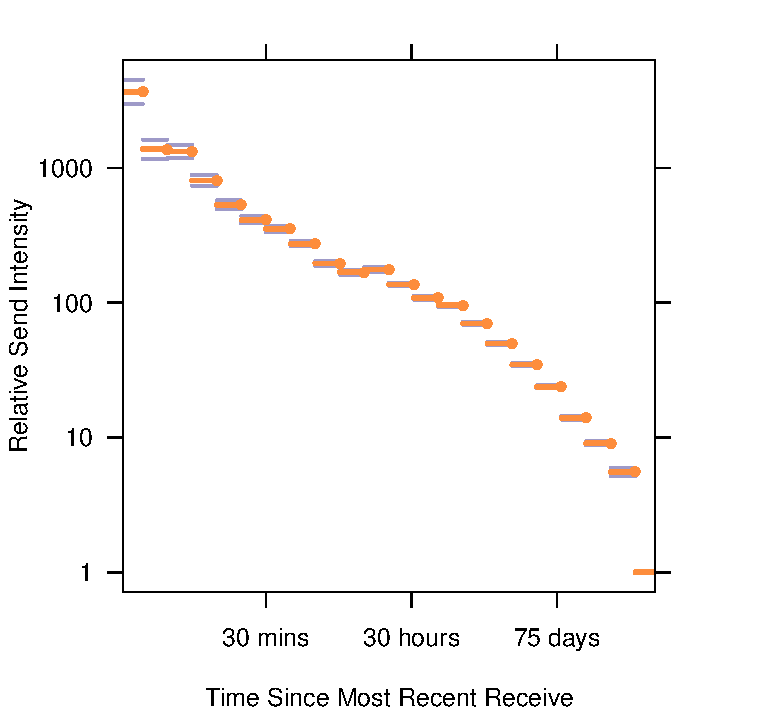
\includegraphics[scale=0.6]{figures/reciprocation-bc}
    \caption{
        \textsc{Reciprocation Effect.}
        Estimated reciprocation effect and standard errors for the
        model described in Section~\ref{S:enron-modeling}.  The solid
        (orange) curve is determined from the 21 estimated coefficients
        for the reciprocation effects at intervals of ``\,$2^l$ hours''
        for $l$ ranging from $-6$ to $14$.  The dashed (purple) curve gives
        one standard error around the estimate.  Read the figure as follows:
        if employee $j$'s most recent message to employee $i$ was 30 minutes
        ago, then $i$ sends to $j$ at about 200 times his baseline rate.
    }\label{F:reciprocation}
\end{figure}

The components of $\beta_0$ corresponding to the static components are not
identifiable, since any $\tilde \beta_0$ satisfying
$\tilde \beta_0^\trans x_t(i,j) = \beta_0^\trans x_t(i,j) + \alpha_t(i)$
gives rise to the same partial likelihood.  We identify $\beta_0$ by
by imposing ``sum-to-zero'' constraints within receiver classes.
This reduces the degrees of freedom in the static coefficients from 144 to
132.

We use history-dependent covariates to capture reciprocation effects.
Specifically, we introduce 21 covariates of the form
\[
    1\{\text{$j$'s most recent message to $i$ was sent in $[t-\delta, t)$\}}.
\]
If, at time $t$, individual $j$ has never sent a message to $i$, then
these covariates are all zero.  The 21 values for the time interval
$\delta$ are of the form ``$2^k$ hours,'' where $k$ is an integer ranging
from $-6$ to $14$.  The shortest time interval is $56.25$ seconds, and the
longest is $1.87$ years.


Table~\ref{T:group-effects} shows the estimated group-level
(static) effects, and Fig.~\ref{F:reciprocation} shows the reciprocation
(dynamic) effects.  Reciprocation is stronger by orders of magnitude,
amplifying the sending rate by between about $10^1$ and $10^3$.  Group level
effects, on the other hand are on the order of $10^{-1}$ to $10^0$.

\begin{table}[h]
    
\begin{tabular}{lrrrr}
    \toprule
    \textbf{Term}
        & \textbf{Df}
        & \textbf{Deviance}
        & \textbf{Resid. Df}
        & \textbf{Resid. Dev} \\
    \midrule
    Null &  &  & 35567 & 358759 \\
    Static & 132 & 63809 & 35435 & 294950 \\
    Dynamic & 21 & 86831 & 35414 & 208119 \\
    \bottomrule
\end{tabular}

    \caption{
        Ad-hoc analysis of deviance for the Enron model.  Residual deviance
        is defined as twice the approximate negative log-partial likelihood
        when messages.  The ``Static'' term contains the group-level effects,
        and the ``Dynamic'' term contains the reciprocation effects.
    }
    \label{T:deviance}
\end{table}

Table~\ref{T:deviance} gives an ad-hoc analysis of deviance for the fitted
model, showing group-level (static) effects account for 18\% of the
residual deviance and reciprocation (dynamic) effects account for 24\%.
If the model fit perfectly, we would expect the residual deviance to be
about equal to the residual degrees of freedom; here, the residual deviance
is about $5.9$ times what we would expect.  Scaling the reported standard errors
by $\sqrt{5.9}$ is an ad-hoc adjustment for this overdispersion.


%\section{Gender Bias in the Enron Dataset}\label{S:gender-bias}
%
%We use the estimated group level effects to quantify the gender bias of
%females and males.  This is defined as follows:
%\begin{enumerate}
%    \item go to the company on the day that it opens, so that there are no
%          reciprocation effects;
%    \item choose a random female employee proportional to how many
%          messages she sent in the dataset;
%    \item \label{I:bias-description-block}
%          block all messages sent to this employee;
%    \item wait for the first message she sends and record the gender
%          of its recipient;
%    \item if the probability of the recipient being female does not
%          agree with the proportion of females in the company ($43 / 156$),
%          then declare there to be gender bias;
%    \item do the same for the first message sent by a male.
%\end{enumerate}
%Step \ref{I:bias-description-block} is necessary because if the chosen
%employee receives a message before she sends one, then her sending
%probabilities will change.
%
%According to Table~\ref{T:gender-effects-dynamic-bc}, females are biased
%towards sending to females, and males are biased towards sending to
%males, even after adjusting for reciprocation effects.  The sub-tables in
%Table~\ref{T:gender-effects} show the impacts of the corrections we have
%made (adjusting for self loops, reciprocation, and multiple recipients).
%As expected, when we adjust for reciprocation, apparent gender bias is less
%pronounced.  Interestingly, the starkest change is for the females,
%indicating that females are more prone to reciprocation than males are
%(we have not explored this interaction in depth).  It turns out that excluding
%self-loops and adjusting for multiple recipients have minor impacts, but we
%could not have known this beforehand.
%
%\begin{table}[h]
%    \label{T:gender-effects}
%    \subtable[Na\"{i}ve Estimates]{
%        
\begin{tabular}{lr@{ }r@{}cr@{ }r}
    \toprule
    & \multicolumn{5}{c}{\textbf{To}} \\
    \cmidrule(l){2-6}
    \textbf{From} & \multicolumn{2}{c}{Female} && \multicolumn{2}{c}{Male} \\
    \midrule
    Female & 0.503 & (0.004) &  & 0.497 & (0.004) \\
    Male & 0.232 & (0.003) &  & 0.768 & (0.003) \\
    \bottomrule
\end{tabular}

%        \label{T:gender-effects-naive}
%    }
%    \subtable[Adjusted for Self-Loops]{
%        
\begin{tabular}{lr@{ }r@{}cr@{ }r}
    \toprule
    & \multicolumn{5}{c}{\textbf{To}} \\
    \cmidrule(l){2-6}
    \textbf{From} & \multicolumn{2}{c}{Female} && \multicolumn{2}{c}{Male} \\
    \midrule
    Female & 0.496 & (0.004) &  & 0.504 & (0.004) \\
    Male & 0.232 & (0.003) &  & 0.768 & (0.003) \\
    \bottomrule
\end{tabular}

%        \label{T:gender-effects-static}
%
%    }
%    \subtable[Adjusted for Reciprocation]{
%        
\begin{tabular}{lr@{ }r@{\,\,}cr@{ }r}
    \toprule
    & \multicolumn{5}{c}{\textbf{To}} \\
    \cmidrule(l){2-6}
    \textbf{From} & \multicolumn{2}{c}{Female} && \multicolumn{2}{c}{Male} \\
    \midrule
    Female & 0.32 & (0.01) &  & 0.68 & (0.01) \\
    Male & 0.23 & (0.03) &  & 0.77 & (0.03) \\
    \bottomrule
\end{tabular}

%        \label{T:gender-effects-dynamic}
%    }
%    \subtable[Adjusted for Multiple Recipients]{
%        
\begin{tabular}{lr@{ }r@{}cr@{ }r}
    \toprule
    & \multicolumn{5}{c}{\textbf{To}} \\
    \cmidrule(l){2-6}
    \textbf{From} & \multicolumn{2}{c}{Female} && \multicolumn{2}{c}{Male} \\
    \midrule
    Female & 0.326 & (0.005) &  & 0.674 & (0.005) \\
    Male & 0.221 & (0.004) &  & 0.779 & (0.004) \\
    \bottomrule
\end{tabular}

%        \label{T:gender-effects-dynamic-bc}
%    }
%    \caption{
%        Estimated gender-level sending preferences.  Probabilities
%        should be compared to the proportions of females and males
%        at the company ($0.276$ and $0.724$, respectively).  Sub-tables
%        show the cumulative estimates after excluding self-loops,
%        including dynamic covariates to adjust for reciprocation, and
%        applying a bias-correction to deal with messages with multiple
%        recipients.
%    }
%\end{table}

\section{Bias Correction for Multiple Recipients}\label{S:bias-correction}



For the Enron corpus the recipient set doesn't grow with the number
of messages, so the bias in the parameter estimate is of order
$1/|\mathcal{J}|$, where $\mathcal{J}$ is the recipient set.  Fortunately,
$|\mathcal{J}|$ is on the order of the square root of the number of messages
in the dataset, so we can correct the bias ($|J|$ is $156$ and there are
$21,365$ messages).  Figure~\ref{F:boot-resid} shows a summary of the bootstrap
residuals from $R = 500$ replicates.  We can see that treating messages with
multiple recipients as multiple single-recipient messages leads to negative
bias in the coefficient estimates.

\begin{figure}
    %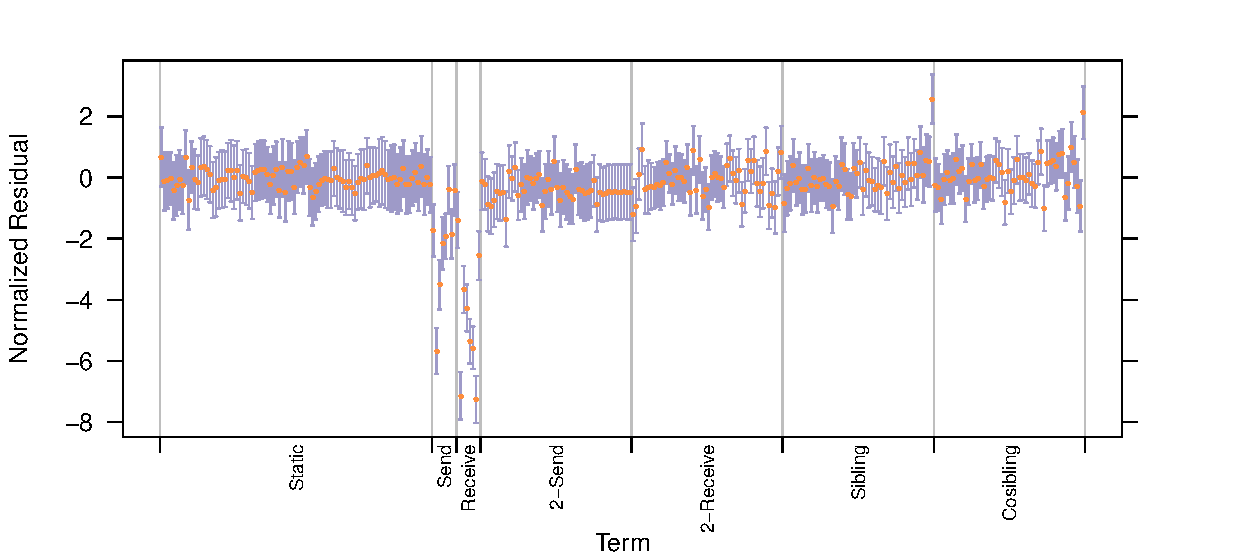
\includegraphics[scale=0.6]{figures/boot-resid}
    \caption{
        \textsc{Enron Bootstrap Residuals.} Summary of bootstrap residuals for
        the coefficients in the Enron dataset, normalized by estimated
        standard errors.  The points (orange) show the means, and the
        error bars (purple) show one standard deviation.  Coefficients
        1--144 are the group-level (static) effects, and coefficients
        145--165 are the reciprocation (dynamic) effects, ordered from
        shortest time interval to longest.  The bias is on the order of
        the standard error, and is near zero for most---but not all---of the
        coefficients.
    }
    \label{F:boot-resid}
\end{figure}


\section{Discussion}\label{S:discussion}

e-mail and other types of ``network'' data are becoming more and more pervasive,
and methods for studying network data are being developed at an accelerating
pace (see Goldenberg et al. and Kolaczyk for recent
overviews~\cite{goldenberg2009survey,kolaczyk2009statistical}).  Unfortunately,
with ``network science'' increasing in popularity, there is a tendency to
shoehorn disparate forms of data into binary ties between actors.  An e-mail
sent between two people is \emph{not} a tie, it is an instantaneous event.
This hasn't discouraged practitioners from forming social networks from
communications data.  One popular approach is to divide the observation period
into time intervals ranging in duration from a week to a month, and then form
a sequence of binary networks by thresholding the number of times pairs of
actors communicate in each interval.  However, as De Choudhury et al. have
shown, the choice of threshold dramatically affects the resulting networks and
downstream analysis~\cite{dechoudhury2010}.  Like
Heard et al.~\cite{heard2010bayesian}, we have avoided these issues by
eschewing network representations entirely.

The models used in this report borrow very little from network science.
Still, they have a lot in common with the agent-based models from that
literature (see \cite{snijders2010introduction} for a recent survey).  Both
conceive of the data as arising from ego-centric decisions made by the actors.
The main difference between agent-based models and our treatment is that we
are dealing with instantaneous events, and they are dealing with ties that
persist in time.  Agent-based models typically involve transitivity (the fact
that your friends' friends are likely to be your friends, too), a behavior
which we have ignored completely.  However, nothing precludes adding covariates
to capture this behavior in our model.

We are not the first to model dyadic interactions with a point processes.
Malmgren et al.\ and Heard et al.\ both use
hidden Markov models for communication activity~\cite{heard2010bayesian,
malmgen2009characterizing}.  Neither of these models model uses covariate
information, and neither uses continuous time.

The foundation of our work is Cox's proportional intensity model and partial
likelihood theory, tools which he first introduced almost forty years ago and
which have been significantly developed since then
\cite{andersen1993statistical,cook2007statistical,cox1972regression,cox1975partial,fleming1991counting,martinussen2006dynamic}.
These tools are used extensively in the context of clinical trials, but have
not yet made an appearance in network data.

We have made two contributions to the theory:
first, we have given asymptotic results which take the limit as the number
of messages grow to infinity instead of assuming a fixed observation interval
and letting the number of subjects grow; second, we have shown that treating
messages with multiple recipients as multiple single-recipient messages leads
to bias in the parameter estimates, but in certain situations this bias can
be corrected. The issue of multiple recipients or interactions with more than
two actors has largely been ignored in the network literature.
Lunag\'omez et al.~\cite{lunagomez2009geometric} have done some relevant
work in the context of graphical models.  We hope the results from
Section~\ref{S:bias-correction} encourage others to take this issue more
seriously.

Our analysis of the Enron data has shown that dynamic effects are important
to e-mail communication, and we expect this to hold broadly for other
types of interactions.  The proportional intensity model with time-varying
covariates is a simple, flexible, and well-established model for incorporating
these effects into the analysis of interaction data.


\section*{Acknowledgement}

The authors thank Joe Blitzstein, Susan Holmes, Art Owen, and Andrew Thomas
for helpful remarks and encouragement.


\appendix

\section{The Enron e-mail Corpus}\label{S:enron-corpus}

The Enron e-mail corpus is a large subset of the e-mail messages sent within the
corporation between November 1998 and June 2002. Enron was an energy company
based in Texas that became notorious in late 2001 for its fraudulent
accounting practices. These practices eventually lead to the resignation of
its CEO, to an external audit into its accounting procedures, to massive
readjustments to its earnings statements, and eventually to its bankruptcy.
Later, many of the top executives were prosecuted and convicted of criminal
fraud and insider trading. As part of the investigation, the Federal Energy
Regulatory Commission (FERC) subpoenaed the e-mail correspondences of the top
employees and posted those not related to the criminal trial to their website
(619,446 messages, roughly 92\% of those subpoenaed).

Leslie Kaelbling, a computer scientist at MIT, purchased the corpus from the
FERC with the intention of making it available to the research community. A
team of researchers at SRI International worked to fix a number of apparent
integrity problems with the data, and then it was released to the public by
William Cohen, at CMU. This is the ``March 2, 2004 Version'' of the dataset.
Later, a former Enron employee requested that one message be removed from the
data; this removal prompted the ``August 21, 2009 Version,'' widely regarded
to be the authoritative version \cite{cohen2009enron}.

Zhou et al. have gone through substantial work to preprocess the Enron corpus
into a useful form \cite{zhou2007strategies}. We rely on their preprocessed
version for our analysis. They reduce the data to the set of e-mails sent by
high-ranking Enron executives, eliminating messages sent by non-employees,
support staff and administrative assistants. They also filter out messages
with missing timestamps. After this culling process, there are 21,635 messages
sent by 156 employees between November 13, 1998 and June 21, 2002. Each e-mail
message has a message body consisting of text, along with header fields
including \texttt{Date}, \texttt{From}, \texttt{To}, \texttt{CC},
\texttt{BCC}, and \texttt{Subject}. The \texttt{From} field always lists a
unique e-mail address, but the \texttt{To}, \texttt{CC}, and \texttt{BCC}
fields sometimes specify multiple recipients. We make no distinction between
\texttt{To}, \texttt{CC}, and \texttt{BCC}, combining them all to determine
the recipients of a message.

We can associate a set of static covariates for each of the 156 individuals in
the dataset. Zhou et al. have extracted the employees' names, departments, and
titles. We use the forenames of the employees to associate genders to the
employees (e.g, John is male, Susan is female). For ambiguously-gendered names
like Dana, Robin, and Sean, we use personal pronouns in the messages to help
code the genders. We code the department as one of three categories: Legal,
Trading, or Other. Finally, we code the position as Senior (CEO, CFO, COO,
Director, Managing Director, VP, President) or Junior (Administrator, Analyst,
Assistant, Attorney, Counsel, Employee, Manager, Specialist, Trader).



\section{Implementation}\label{S:implementaiton}

For small-to-medium datasets, one can fit proportional intensity models
using \texttt{coxph} from the \texttt{survival} package for R
\cite{therneau2009survival}.  Unfortunately, with 156 senders and
over $20,000$ messages, the Enron dataset is too large for the package
to handle.  We instead wrote custom software to maximize the partial
likelihood.

Suppose $(t_1, i_1, j_1), \ldots, (t_n, i_n, j_n)$ is the sequence of observed
messages, where tuple $(t,i,j)$ indicates that at time $t$, sender $i$ sent a
message to receiver $j$.  Define the following message sets:
\begin{align*}
  \mathcal{M}_t(i,j)
    &= \{ m : t_m \leq t, \, i_m = i, \, j_m = j \}, \\
  \mathcal{M}_t(i)
    &= \cup_{j \in \mathcal{J}} \mathcal{M}_t(i,j), \\
  \mathcal{M}_t
    &= \cup_{i \in \mathcal{I}} \mathcal{M}_t(i).
\end{align*}
The partial likelihood factors into a product of terms, one for each sender:
\begin{align*}
    \mathit{PL}_t(\beta)
        &=
        \,\,
        \prod_{i \in \mathcal{I}}
            \,\,
            \mathit{PL}_t(\beta, i), \\
    \mathit{PL}_t(\beta, i)
        &=
        \!\!\!\!
        \prod_{m \in \mathcal{M}_t(i)}
            \!\!\!
            \frac{w_{t_m} (\beta, i, j_m)}
                 {W_{t_m}(\beta, i)}.
\end{align*}
This factorization allows us to compute $\log \mathit{PL}_t(\beta)$ and
its derivatives by computing the sender-specific terms in parallel and
then adding them together.

The sender-specific log-partial likelihood and its derivatives are
\begin{align*}
    \log \mathit{PL}_t(\beta, i)
        &=
        \!\!\!\!
        \sum_{m \in \mathcal{M}_t(i)}
            \!\!\!
            \beta^\trans
            x_{t_m}\!(i, j_m)
            \,
            -
            \,
            \log W_{t_m}\!(\beta, i), \\
    \nabla [ \log \mathit{PL}_t(\beta, i) ]
        &=
        \!\!\!\!
        \sum_{m \in \mathcal{M}_t(i)}
            \!\!\!
            x_{t_m}\!(i,j_m)
            \,
            -
            \,
            \frac{1}{W_{t_m}\!(\beta,i)}
                \sum_{j \in \mathcal{J}(i)}
                    w_{t_m}\!(\beta,i,j) \,
                    x_{t_m}\!(i,j), \\
    \begin{split}
    \nabla^2 [ \log \mathit{PL}_t(\beta, i) ]
        &=
        -
        \!\!\!\!
        \sum_{m \in \mathcal{M}_t(i)}
            \!\!
            \bigg\{
            \frac{1}{W_{t_m}\!(\beta,i)}
            \sum_{j \in \mathcal{J}(i)}
                w_{t_m}\!(\beta,i,j) \,
                \big[
                    x_{t_m}\!(i,j)
                \big]^{\otimes 2} \\
        &\qquad\qquad\qquad-
            \Big[
                \frac{1}{W_{t_m}\!(\beta,i)}
                \sum_{j \in \mathcal{J}(i)}
                    w_{t_m}\!(\beta,i,j) \,
                    x_{t_m}\!(i,j)
            \Big]^{\otimes 2}
            \bigg\},
    \end{split}
\end{align*}
where $a^{\otimes 2} = a a^\trans$.  When $x_t(i,j)$ is constant over time,
there are sufficient statistics for $\beta$ and these formulas reduce.
Otherwise, computing $\log \mathit{PL}_t(\beta,i)$ and its derivatives
requires iterating over all messages, potentially taking time
$\Oh(|\mathcal{M}_t(i)| \cdot |\mathcal{J}(i)| \cdot p^2)$.
The serial computation time for computing the full partial likelihood
and its derivatives is $\Oh(M \cdot J \cdot p^2)$.
For the Enron data, $M \approx 20,\!000$, $J \approx 150$,
and $p \approx 200$.  This is relatively small by modern standards.  Often
$M$ on the order of $10^9$ and $J$ on the order of $10^6$.  Computations
taking time $\Oh(M \cdot J)$ are prohibitive for large datasets.

Taking advantage of sparsity, the serial time for computing the
gradient reduces to $\Oh(M \cdot p + I \cdot J)$.   Our implementation
uses a gradient-based optimization method (the
Broyden-Fletcher-Goldfarb-Shanno algorithm \cite{nocedal2006numerical}) to
compute the MPLE in linear time.

Assume for the remainder that
$\mathcal{J}_t(i) = \mathcal{J}(i)$, i.e., that $\mathcal{J}_t(i)$ is
constant.  Decompose $x$ into its static (non time-varying) and dynamic parts:
\[
    x_t(i,j)
        = x_0(i,j) + d_t(i,j).
\]
Typically, the dynamic part, $d_t(i,j)$, is sparse, with at most $\bar p$
nonzero components.  Moreover $d_t(i,j)$ is zero for most $(i,j)$
pairs---often $d_t(i,j)$ is zero unless $i$ and $j$ have exchanged
messages in the past.  Let
\[
    \mathcal{\bar J}(i)
        =
        \{
            j \in \mathcal{J}(i) : d_t(i,j) \neq 0
            \,\,
            \text{for some $t$}
        \}.
\]
Assume $|\mathcal{\bar J}(i)| \ll |\mathcal{J}(i)|$ and that
computing $d_t(i,j)$ takes amortized time $\Oh(\bar p)$ for each
$(t,i,j)$ triple.

Notice
\begin{align*}
    w_{t}(\beta,i,j)
        &=
            w_{0}(\beta,i,j)
            \cdot
            \exp\{ \beta^\trans d_t(i,j) \}, \\
    W_{\beta,t}(i)
        &=
            W_{0}(\beta,i)
            +
            \sum_{j \in \mathcal{\bar J}(i)}
                w_{t}(\beta,i,j) - w_{0}(\beta,i,j)
\end{align*}
It takes time $\Oh(|\mathcal{J}(i)| \cdot p)$ to compute the values of
$W_{0}(\beta,i)$ and $w_{0}(\beta,i,j)$ for any $i$ and all
$j$ in $\mathcal{J}(i)$; once these values are known, computing the values
of $W_{t}(\beta,i)$ and $w_{t}(\beta,i,j)$ takes time
\(
    \Oh(|\mathcal{\bar J}(i)| \cdot \bar p).
\)
Since
\[
    \sum_{m\in \mathcal{M}_t(i)}
        x_{t_m}\!(i,j_m)
        =
            \sum_{j \in \mathcal{J}(i)}
                |\mathcal{M}_t(i,j)| \, x_0(i,j)
            \,\,\,
            +
            \sum_{m \in \mathcal{M}_t(i)}
                d_{t_m}\!(i,j),
\]
%computing sum on the left hand side takes time
%\(
%    \Oh(|\mathcal{M}_t(i)| \cdot \bar p + |\mathcal{J}(i)| \cdot p);
%\)
computing $\log \mathit{PL}_t(\beta, i)$ takes time
\(
    \Oh(
        |\mathcal{M}_t(i)| \cdot |\mathcal{\bar J}(i)| \cdot \bar p
        +
        |\mathcal{J}(i)| \cdot p
    ).
\)

The second term in the gradient is
\begin{multline*}
    \sum_{m \in \mathcal{M}_t(i)}
        \frac{1}{W_{t_m}\!(\beta,i)}
        \sum_{j \in \mathcal{J}(i)}
            w_{t_m}\!(\beta,i,j)
            \,
            x_{t_m}\!(i,j) \\
    =
    \sum_{j \in \mathcal{J}(i)}
    \bigg[
        \sum_{m \in \mathcal{M}_t(i)}
            \frac{w_{t_m}\!(\beta,i,j)}{W_{t_m}\!(\beta,i)}
    \bigg]
    \cdot
    x_0(i,j) \\
    +
    \sum_{m \in \mathcal{M}_t(i)}
        \frac{1}{W_{t_m}\!(\beta,i)}
        \sum_{j \in \mathcal{\bar J}(i)}
            w_{t_m}\!(\beta,i,j)
            \,
            d_{t_m}\!(i,j).
\end{multline*}
Also,
\[
    \sum_{m \in \mathcal{M}_t(i)}
        \frac{w_{t_m}\!(\beta,i,j)}{W_{t_m}\!(\beta,i)}
    =
        w_{0}(\beta,i,j)
        \cdot
        \sum_{m \in \mathcal{M}_t(i)}
            \frac{
                \exp\{\beta^\trans d_{t_m}\!(i,j) \}
            }{
                W_{t_m}\!(\beta,i)
            };
\]
the latter term is constant when $j \notin \mathcal{\bar J}(i)$.
Organizing the computations as suggested by these formula,
the additional overhead for computing the gradient of
$\log \mathit{PL}_t(\beta,i)$ is
\(
    \Oh(
        |\mathcal{M}_t(i)| \cdot |\mathcal{\bar J}(i)| \cdot \bar p
        +
        |\mathcal{J}(i)| \cdot p
    )
\).
This is the same computational complexity as for computing
$\log \mathit{PL}_t(\beta,i)$.


Suppose $|\mathcal{J}(i)| \leq J$, $|\mathcal{\bar J}(i)| \leq \bar J$,
and $|\mathcal{M}_t(i)| \leq M$.  By organizing the computations as described
above, we can compute $\log \mathit{PL}_t(\beta)$ and its gradient in serial
time
\(
    \Oh(
        | \mathcal{I} |
        \cdot
        M
        \cdot
        \bar J
        \cdot
        \bar p
        +
        |\mathcal{I}| \cdot J \cdot p
    ).
\)
With $\Oh(|\mathcal{I}|)$ processors, we can compute these quantities in time
\(
    \Oh(
        M \cdot \bar J \cdot \bar p
        +
        J \cdot p
        +
        |\mathcal{I}| \cdot p
    ).
\)

\section{Proofs of MPLE Results}\label{S:MPLE-consistency-proofs}

\begin{lemma}\label{L:adapted-martingale}
$\tilde U_\alpha^{(n)}(\beta_0)$ from *** is a square-integrable martingale
adapted to
\(
    \mathcal{\tilde F}^{(n)}_\alpha
        =
        \mathcal{F}_{\tau_{\lfloor \alpha n \rfloor}}.
\)
\end{lemma}

\begin{proof}
The conditional expectation property holds provided
\(
    \E[ U_{\tau_{n}}(\beta_0) \mid \mathcal{F}_{\tau_{n-1}} ]
        = U_{\tau_{n-1}}(\beta_0).
\)
Define $K = \sup_{t,i,j} \| x_{t}(i,j) \|$.
Note that $\|H_{t}(i,j)\| \leq 2 K$.  Thus,
\begin{align*}
    \| U_{t \wedge \tau_n} (\beta_0) \|
        &\leq
            2 K
            \big(
                N_{t \wedge \tau_n}
                +
                \Lambda_{t \wedge \tau_n}
            \big), \\
\intertext{so that}
    \E \left[
        \sup_t
        \| U_{t \wedge \tau_n} (\beta_0) \|^2
    \right]
        &\leq
            8 \cdot \big(\E K^2\big)^{1/2} \cdot
            \big(
              \E N_{\tau_n}^2
              +
              \E \Lambda_{\tau_n}^2
            \big)^{1/2}.
\end{align*}
By assumption A\ref{A:square-int}, $\E K^2$ is finite, and by construction,
$N_{\tau_n}$ is bounded.  Since $N_{t \wedge \tau_n}$ is a counting process,
$\E \Lambda_{\tau_n}^2$ is finite, too
(this follows from results in Section 2.3 of Fleming and Harrington
\cite{fleming1991counting}).  Thus, $U_{t \wedge \tau_n}(\beta_0)$
is uniformly integrable.  The Optional Sampling Theorem now applies to
give the conditional expectation property of $\tilde U^{(n)}(\beta_0)$.  For
square integrability, note
\(
    \sup_{1 \leq m \leq n}
    \E \| U_{\tau_m} \|^2
        \leq
        \E \left[
           \sup_t
           \| U_{t \wedge \tau_n} (\beta_0) \|^2
        \right].
\)
\end{proof}

\begin{lemma}\label{L:Lindeberg-condition}
The Lindeberg condition is that for any positive $\varepsilon$,
\[
    \frac{1}{n}
    \sum_{i,j}
    \int_{0}^{\tau_n}
        \| H_s(i,j) \|^2
        \, 1\{\| H_s(i,j) \| > \sqrt{n} \varepsilon \}
        \, d\Lambda_s(i,j)
        \toP
        0.
\]
\end{lemma}

\begin{proof}
With $K = \sup_{t,i,j} \| x_t(i,j)\|$ as above, the integral is bounded by
\(
    4 \, K^2 \, 1\{n^{-1/2} K > \varepsilon / 2\}
    \cdot
    \frac{\Lambda_{\tau_n}}{n}.
\)
Since $\E K^2 < \infty$, the first term converges to zero in probability.
Since $\E \Lambda_{\tau_n} = \E N_{\tau_n} = n$, the product of the two also
converges to zero in probability.  Thus, the Lindeberg condition is satisfied.
\end{proof}


\begin{lemma}\label{L:Lenglart}
Foo
\end{lemma}

\begin{proof}
Lenglart's Inequality and assumption~A\ref{A:message-times-finite} imply that for
any positive $\rho$ and $\delta$,
\begin{multline*}
    \mathbb{P}\left\{
        \sup_{t \in [0,\tau_n]}
        \left\|
            \frac{1}{n}
            \sum_{i}
            \int_{0}^{t}
                V_s(\beta_0, i) \, dM_s(i)
        \right\|
        \geq \rho
    \right\} \\
    \leq
    \frac{\delta}{\rho^2}
    +
    \mathbb{P}\left\{
        \frac{1}{n^2}
        \sum_{i}
        \int_{0}^{\tau_n}
            \| V_s (\beta_0, i) \|^2
            \, d\Lambda_s(i)
        \geq
        \delta
    \right\}.
\end{multline*}
(see Fleming and Harrington's Cor.~3.4.1 for a related proof
\cite{fleming1991counting}).    As in the proof of
Lemma~\ref{L:adapted-martingale}, set $K = \sup_{t,i,j} \| x_t(i,j) \|$.
The sum in the second term is bounded by
$\frac{K^4}{n} \cdot \frac{\Lambda_{\tau_n}}{n}$.  Since $n^{-1/2} K^2 \toP 0$
and $\E \Lambda_{\tau_n} = n$, the right hand side of the inequality converges
to $\frac{\delta}{\rho^2}$.  Since $\delta$ is arbitrary, the right hand side
must converge to zero.  This proves that the second term in the bound on
\(
    \left\|
        \tfrac{1}{n} I_{\tau_{\lfloor \alpha n \rfloor}}(\hat \beta_n)
        -
        \Sigma_{\alpha} (\beta_0)
    \right\|
\)
converges to zero uniformly in $\alpha$, concluding the proof.
\end{proof}

\subsection{Proof of Theorem~\ref{T:consistency}}\label{S:proof-consistency}

We follow Haberman's approach to proving
consistency, which relies on Kantorovich's analysis
of Newton's method.  Tapia gives an elementary proof of the Kantorovich
Theorem~\cite{haberman1977maximum,kantorovich1952functional,tapia1971kantorovich}.
We state a weak form of the result as a lemma.

\begin{lemma}[Kantorovich Theorem]\label{L:kantorovich}
    Let $P(x) = 0$ be a general system of nonlinear equations, where $P$ is
    a map between two Banach spaces.  Let $P'(x)$ denote the Jacobian
    (Fr\'echet differential) of $P$ at $x$, assumed to exist in $D_0$,
    a convex open neighborhood of $x_0$.  Assume the following:
    \begin{enumerate}[(i)]
        \item $\| [P'(x_0)]^{-1} \| \leq B$,
        \item $\| [P'(x_0)]^{-1} P(x_0) \| \leq \eta$,
        \item $\| P'(x) - P'(y) \| \leq K \| x - y \|$,\quad
            for all $x$ and $y$ in $D_0$,
    \end{enumerate}
    with $h = B K \eta \leq \tfrac{1}{2}$.

    Let $\Omega_\ast = \{ x : \| x - x_0 \| \leq 2 \eta \}$.
    If $\Omega_\ast \subset D_0$, then the Newton iterates,
    $x_{k+1} = x_k - [P'(x_k)]^{-1} P(x_k)$, are well defined, remain
    in $\Omega_\ast$, and converge to $x^\ast$ in $\Omega_\ast$ such
    that $P(x^\ast) = 0$.  In addition,
    \[
        \| x^\ast - x_k \|
            \leq
                \frac{\eta}{h}
                \frac{(2h)^{2^k}}{2^k},
        \qquad
        k = 0, 1, 2, \ldots.
    \]
\end{lemma}

\begin{proof}[Proof of Theorem~\ref{T:consistency}]
Set $U_t(\cdot)$ and $I_t(\cdot)$ to be the gradient and negative
Hessian of the log partial likelihood, as defined in
(\ref{E:log-pl-gradient}--\ref{E:log-pl-neg-hessian}).  Since
$I_t(\beta)$ is a sum of rank-one matrices with positive weights,
it is positive semi-definite, and $\log \mathit{PL}_t(\cdot)$ is
a concave function.  By the assumption that the smallest
eigenvalue of $\Sigma_1(\cdot)$ is bounded away from zero in a neighborhood
of $\beta_0$, for $n$ sufficiently large, if $\log \mathit{PL}_t(\cdot)$ has a 
local minimum in that neighborhood then it must be the unique global maximum.

We find the local maximum by applying Newton's method to the
gradient of $\tfrac{1}{n} \log \mathit{PL}_{\tau_n}(\cdot)$, taking
$\beta_0$ as the initial iterate.  Define
\[
   Z_n = -[\tfrac{1}{n} I_{\tau_n}(\beta_0)]^{-1} [ \tfrac{1}{n} U_{\tau_n}(\beta_0)].
\]
The first Newton iterate, $\beta_{n,1}$ is equal to $\beta_0 - Z_n$.
Part (ii) of Theorem~\ref{T:score-fisher} and the
assumptions of the theorem imply $[\tfrac{1}{n} I_{\tau_n}(\beta_0)]^{-1}$
exists for $n$ large enough so that $Z_n$ is well-defined.  
Moreover, Part (i) of Theorem~\ref{T:score-fisher} and Slutzky's Theorem imply
$Z_n \toP 0$ and
$\sqrt{n} \, Z_n \tod \Normal(0,\, [\Sigma_1(\beta_0)]^{-1})$.


Apply Kantorovich's Theorem to bound $\| \hat \beta_n - \beta_0 \|$
and $\| \hat \beta_n - \beta_{n,1} \|$.  By assumption, there exists
a neighborhood of $\beta_0$, say $D_0$, and finite $K$ and $B$, such that
\(
    \|
        \frac{1}{n} I_{\tau_n} (\beta)
        -
        \frac{1}{n} I_{\tau_n}(\beta')
    \|
    \leq
    K
    \|
        \beta
        -
        \beta'
    \|
\)
and
\(
    \| \frac{1}{n} [I_{\tau_n}(\beta_0)]^{-1} \| \leq B
\)
for $\beta, \beta' \in D_0$.
Define $\eta_n = \| Z_n \|$ and $h_n = B K \eta_n$, noting that $h_n$ and
$\eta_n$ are size $\OhP(n^{-1/2})$.  Thus, for $n$ large enough, the
\begin{enumerate}[(i)]
    \item $\| \hat \beta_n - \beta_0 \| \leq 2 \, \eta_n \toP 0$,
    \item
        \(
            \sqrt{n} \, \| \hat \beta_n - (\beta_0 - Z_n) \|
            \leq
            2 \sqrt{n} \, \eta_n \, h_n
            \toP 0.
        \)
\end{enumerate}
Thus, $\hat \beta_n \toP \beta_0$, and $\sqrt{n} (\hat \beta_n - \beta_0)$
and $\sqrt{n} \, Z_n$ converge weakly to the same limit.
\end{proof}

\section{Proofs of Multiple Recipient Results}\label{S:multiple-recipient-proofs}

\begin{lemma}\label{L:coupling-prob-bound}
Using the notation and assumptions of 
Theorem~\ref{T:log-pl-multiple-approx-error},
\[
    \mathbb{P}^\ast_{t,\beta,i;L}
    \Big\{
        (j_1, \ldots, j_L)
            \neq
            (\tilde \jmath_1, \ldots, \tilde \jmath_L)
    \Big\}
        \leq
        {L \choose 2}
        \cdot
        \frac{\exp\{4 K \, \| \beta \|\}}{| \mathcal{J}_t(i) |},
\]
where $K = \sup_t \| x_t(i,j) \|$.
\end{lemma}
\begin{proof}
\begin{align*}
    \mathbb{P}^\ast_{t,\beta,i;L}
    \Big\{
        (j_1, \ldots, j_L)
            \neq
            (\tilde \jmath_1, \ldots, \tilde \jmath_L)
    \Big\}
        &=
        \mathbb{P}^\ast_{t,\beta,i;L}
        \Big\{
            \text{$\tilde \jmath_1, \ldots, \tilde \jmath_L$ has a duplicate}
        \} \\
        &\leq
        \sum_{k \leq l}
            \mathbb{P}^\ast_{t,\beta,i;L}
            \Big\{
                \tilde \jmath_k = \tilde \jmath_l
            \Big\} \\
        &=
            {L \choose 2}
            \sum_{j \in \mathcal{J}_t(i)}
                \Big[
                    \frac{
                        w_t(\beta, i, j)
                    }{
                        \sum_{j' \in \mathcal{J}_t(i)} w_t(\beta, i, j')
                    }
                \Big]^2.
\end{align*}
Note
\(
    \exp\{-K \, \| \beta \|\}
        \leq w_t(\beta,i,j)
        \leq \exp\{K \| \, \beta \|\},
\)
so that
\[
    \sum_{j \in \mathcal{J}_t(i)}
        \Big[
            \frac{
                w_t(\beta, i, j)
            }{
                \sum_{j' \in \mathcal{J}_t(i)} w_t(\beta, i, j')
            }
        \Big]^2.
    \leq
        \frac{\exp\{4 K \, \| \beta \|\}}{| \mathcal{J}_t(i) |}.
    \qedhere
\]    
\end{proof}


\begin{lemma}\label{L:hessian-approx-bound}
Using the notation and assumptions of 
Theorem~\ref{T:log-pl-multiple-approx-error},
\begin{multline*}
    \Big\|
        \nabla^2\big[ \log \widetilde{\mathit{PL}}_t(\beta) \big]
        -
        \nabla^2\big[ \log \mathit{PL}_t(\beta) \big]
    \Big\| \\
        \leq
            2K^2
            \exp\{4 K \| \beta \|\}
            \cdot
            \sum_{t_m \leq t}
                \frac{|J_m|^3 \, (|J_m| - 1)}{|\mathcal{J}_{t_m}(i_m)|}.
\end{multline*}    
\end{lemma}
\begin{proof}
The argument is similar to the bound on the difference in gradients in
the proof of Theorem~\ref{T:log-pl-multiple-approx-error}.  The Hessians of 
the weights are
\begin{align}
    \begin{split}
    V_t(\beta,i;L)
        &=
        \nabla^2 \big[  \log W_t(\beta, i; L) \big] \\
        &=
        \frac{1}{W_t(\beta,i;L)}
        \sum_{\substack{J \subseteq \mathcal{J}_t(i), \\
                        |J| = L}}
            w_t(\beta,i,J)
            \Big[
                X_t(i,J)
                -
                E_t(\beta,i;L)
            \Big]^{\otimes 2},
    \end{split} \\
    \begin{split}
    \widetilde V_t(\beta,i;L)
        &=
        \nabla^2 \big[ \log \widetilde W_t(\beta,i;L) \big] \\
        &=
        L
        \cdot
        \frac{
            \sum_{j \in \mathcal{J}_t(i)}
                w_t(\beta, i, j)
                \Big[ x_t(i,j) - \tfrac{1}{L} \widetilde E_t(\beta,i;L) \Big]^{\otimes 2}
        }{
            \sum_{j \in \mathcal{J}_t(i)}
                w_t(\beta, i, j)
        }.
    \end{split}
\end{align}
The first is the covariance matrix of $\sum_{l=1}^L x_t(i,j_l)$ under
$\mathbb{P}_{t,\beta,i;L}$; the second is the covariance matrix of the same
quantity under $\tilde{\mathbb{P}}_{t,\beta,i;L}$.
The result follows in the same manner as in the proof of 
Theorem~\ref{T:log-pl-multiple-approx-error}.
The relevant intermediate bounds is
\[
    \Big\| V_{t}(\beta, i; L) - \widetilde{V}_t(\beta, i; L) \Big\|
        \leq
        2\, K^2 \, L^3 \, (L - 1)
        \,
        \frac{\exp\{4 K \, \| \beta \|\}}{| \mathcal{J}_t(i) |}.
    \qedhere
\]
\end{proof}


\begin{proof}[Proof of Theorem~\ref{T:mple-approx-error}]

We know that Newton's method applied to
$\tfrac{1}{n}\log \widetilde{\mathit{PL}}_{\tau_n}(\cdot)$ converges to
$\tilde \beta_n$ after enough iterations.  We use $\hat \beta_n$ as the
initial iterate and use the Kantorovich Theorem (Lemma~\ref{L:kantorovich})
to bound $\|\tilde \beta_n - \hat \beta_n\|$.

In the notation of the lemma, $P(\cdot)$ is the gradient of
$\tfrac{1}{n} \log \widetilde{\mathit{PL}}_{\tau_n}(\cdot)$ and $P'(\cdot)$ is its Hessian.
Singe $G_n/n \toP 0$, assumptions (i) and (iii) hold for
some finite $B$ and $K$ uniformly for $n$ large enough with arbitrarily
high probability by
Theorem~\ref{T:log-pl-multiple-approx-error}
and the assumptions on $\tfrac{1}{n} \nabla^2 [\log {\mathit{PL}}_{\tau_n}(\cdot)]$.
Likewise, for large enough $n$,
\(
    \Big\|
        \nabla^2\big[
            \tfrac{1}{n}
            \log \widetilde{\mathit{PL}}_{\tau_n}(\hat \beta_{\tau_n})
        \big]
    \Big\|
\)
is uniformly bounded away from zero with arbitrarily high probability.
Equivalently, the norm of the inverse Hessian is bounded.

Set
\[
    \eta_n =
    \Big\|
        \Big[
            \nabla^2\big[
                \tfrac{1}{n}
                \log \widetilde{\mathit{PL}}_{\tau_n}(\hat \beta_{\tau_n})
            \big]
        \Big]^{-1}
        \Big[
            \nabla\big[
                \tfrac{1}{n}
                \log \widetilde{\mathit{PL}}_{\tau_n}(\hat \beta_{\tau_n})
            \big]
        \Big]
    \Big\|
\]
and set $h_n = B K \eta_n$.
Since $\nabla\big[\log {\mathit{PL}}_{\tau_n}(\hat \beta_{\tau_n})\big] = 0$,
Theorem~\ref{T:log-pl-multiple-approx-error} and the boundedness of the
inverse Hessian give us that $\eta_n = \OhP(G_n/n)$.  Therefore, for $n$
large enough,
\[
    \| \tilde \beta_n - \hat \beta_n \|
        \leq \frac{\eta_n}{h}\frac{(2h)^{2^0}}{2^0}
        = 2 \eta_n
        = \OhP(G_n/n).
    \qedhere
\]
\end{proof}


\bibliographystyle{imsart-number}
\bibliography{iproc-sources}

\end{document}
